\documentclass[a4paper,12pt,oneside]{report}

\newif\ifrelease % new boolean variable release. True = include some fancy content
\releasefalse % and set it

\usepackage[english]{babel}
\usepackage[utf8]{inputenc}
\usepackage[T1]{fontenc}
\usepackage{amsmath}
\usepackage{amssymb}
\usepackage{epsfig}
\usepackage{graphicx}
\usepackage{enumitem} % so that spacing for lists can be easily set, resume option etc
\ifrelease
	\usepackage{pdfpages}
\fi
\usepackage[hyphens]{url} % the package is not needed, it needes just to set the parameter
\usepackage[pagebackref=true]{hyperref} % tento balicek by mel byt na konci baliku!

\hypersetup{
	pdfauthor={Matej Laitl},
	pdftitle={Implementation environment for Bayesian filtering algorithms}
}

%% Nastavení zrcadla sazby
\usepackage{calc}
\setlength{\textheight}{9in}
\setlength{\textwidth}{6in}
\setlength\oddsidemargin{(\paperwidth-\textwidth)/2 - 1in}
\setlength\evensidemargin{(\paperwidth-\textwidth)/2 - 1in}
\setlength\topmargin{(\paperheight-\textheight-\headheight-\headsep-\footskip)/2 - 1in}

%\parindent=0pt % odsazení 1. řádku odstavce
\parskip=4pt   % mezera mezi odstavci

% set that list should not have vertical space
\setlist{nolistsep}
\setlist[1]{leftmargin=\parindent} % set indentation to level 1 lists to be same as paragraph indent

\ifrelease
	\hypersetup{pdfborder={0 0 0}} % no borders around links
\else
	\hypersetup{colorlinks=true} % colour links instead of borders
\fi

% definitions of our own commands:
\newcommand{\pdf}{probability density function}
\newcommand{\pdfs}{probability density functions}
\newcommand{\supp}{\operatorname{supp}}
\newcommand{\dx}{\mathrm{d}x}


\begin{document}

\ifrelease
	\newcommand{\cvut}{České vysoké učení technické v~Praze}
\newcommand{\fjfi}{Fakulta jaderná a fyzikálně inženýrská}
\newcommand{\km}{Katedra matematiky}
\newcommand{\obor}{Inženýrská Informatika}
\newcommand{\zamereni}{Softwarové inženýrství a matematická informatika}

\newcommand{\nazevcz}{Prostředí pro implementaci algoritmů Bayesovské filtrace}
\newcommand{\nazeven}{Implementation environment for Bayesian filtering algorithms}
\newcommand{\autor}{Matěj Laitl}
\newcommand{\rok}{2011}
\newcommand{\vedouci}{Ing. Václav Šmídl, Ph.D.}

\newcommand{\pracovisteVed}{Oddělení adaptivních systémů \\
	Ústav teorie informace a automatizace \\
	Akademie věd České republiky}
\newcommand{\konzultant}{---}
\newcommand{\pracovisteKonz}{}

\newcommand{\klicova}{Bayesovská filtrace, softwarová analýza, Python, Cython} % TODO: dalsi?
\newcommand{\keyword}{Bayesian filtering, software analysis, Python, Cython}
% Abstrakt práce: (cca 7 vět, min. 80 slov)
\newcommand{\abstrCZ}{Bayesovská filtrace je velmi použitelný přístup k odhadování dynamických
systémů, který má mnoho aplikací v robotice, environmentálních simulacích a dalších oborech. Tato
práce předkládá popis Kalmanova filtru, částicového filtru a marginalizovaného částicového filtru,
který využívá myšlenky obou předchozích. Poté je provedena softwarová analýza, která má za úkol
určit nejvhodnější implementační prostředí pro softwarovou knihovnu poskytující metody Bayesovské
filtrace. Nejprve jsou posouzeny obecné přístupy k vývoji software, z nichž je jako nejpoužitelnější
zvolen objektově orientovaný, následuje porovnání programovacích jazyků C++, MATLAB a Python.
Python zvítězí a v je něm napsána knihovna pro Bayesovskou filtraci nazvaná PyBayes; nakonec je
dosaženo výrazného zrychlení Pythonového kódu použitím Cythonu.}
\newcommand{\abstrEN}{Bayesian filtering is a vital approach to dynamic system estimation that has
wide applications in robotics, environmental simulations and much more. This text briefly introduces
the Kalman filter, the particle filter and the marginalized particle filter which combines ideas of
both. Software analysis is performed with the aim to identify the most suitable implementation
environment for a software library for Bayesian filtering. Various paradigms of software development
and are discussed among which the object-oriented programming is chosen; C++, MATLAB and Python
languages are evaluated. Python is determined most appropriate and a Python software library named
PyBayes is developed; dramatic performance gains are measured when Cython is used to speed up
Python.}

%%% zde zacina kresleni dokumentu

% titulní strana
\thispagestyle{empty}

\begin{center}
	{\Large  \bf  \cvut\\[2mm] \fjfi }
	\vspace{10mm}

	\begin{tabular}{c}
	{\bf \km}\\
	{\bf Obor: \obor}\\
	{\bf Zaměření: \zamereni}
	\end{tabular}

	\vspace{10mm} \epsfysize=20mm  \epsffile{cvut-logo-bw-600} \vspace{15mm}

	{\LARGE
	\textbf{\nazevcz}
	\par}

	\vspace{5mm}

	{\LARGE
	\textbf{\nazeven}
	\par}

	\vspace{30mm}
	{\Large BAKALÁŘSKÁ PRÁCE}

\end{center}

\vfill
{\large
\begin{tabular}{rl}
Vypracoval: & \autor\\
Vedoucí práce: & \vedouci\\
Rok: & \rok
\end{tabular}
}

% zadání bakalářské práce
\newpage
\thispagestyle{empty} Před svázáním místo téhle stránky \fbox{vložíte zadání práce} s podpisem
děkana (bude to jediný oboustranný list ve Vaší práci) !!!!

% prohlášení
\newpage
\thispagestyle{empty}
~
\vfill


{\bf Prohlášení}

\vspace{0.5cm}
Prohlašuji, že jsem svou bakalářskou práci vypracoval samostatně a použil jsem pouze podklady
(literaturu, projekty, SW atd.) uvedené v přiloženém seznamu.

\vspace{5mm}V Praze dne ....................\hfill
    \begin{tabular}{c}
    ........................................\\
    \autor
    \end{tabular}

% poděkování
\newpage
\thispagestyle{empty}
~
\vfill

{\bf Poděkování}

\vspace{5mm}
Děkuji Ing. Václavu Šmídlovi, Ph.D. za vedení mé bakalářské práce, velmi prozíravě položené
softwarové otázky a za poukázání na softwarové projekty (Cython, Sphinx, \ldots), které se ukázaly
být klíčové pro moji bakalářskou práci a softwarový projekt.

\begin{flushright}
\autor
\end{flushright}

% strana s abstraktem
\newpage
\thispagestyle{empty}

\newbox\odstavecbox
\newlength\vyskaodstavce
\newcommand\odstavec[2]{%
    \setbox\odstavecbox=\hbox{%
         \parbox[t]{#1}{#2\vrule width 0pt depth 4pt}}%
    \global\vyskaodstavce=\dp\odstavecbox
    \box\odstavecbox}
\newcommand{\delka}{120mm}

\noindent\begin{tabular}{@{}ll}
  {\em Název práce:} & ~ \\
  \multicolumn{2}{@{}l}{\odstavec{\textwidth}{\bf \nazevcz}} \\[5mm]
  {\em Autor:} & \autor \\[5mm]
  {\em Obor:} & \obor \\
  {\em Druh práce:} & Bakalářská práce \\[5mm]
  {\em Vedoucí práce:} & \odstavec{\delka}{\vedouci \\ \pracovisteVed} \\[5mm]
  {\em Konzultant:} & \odstavec{\delka}{\konzultant \\ \pracovisteKonz} \\[5mm]
  \multicolumn{2}{@{}l}{\odstavec{\textwidth}{{\em Abstrakt:} ~ \abstrCZ \\ }} \\[5mm]
  {\em Klíčová slova:} & \odstavec{\delka}{\klicova} \\[10mm]

  {\em Title:} & ~\\
  \multicolumn{2}{@{}l}{\odstavec{\textwidth}{\bf \nazeven}}\\[5mm]
  {\em Author:} & \autor \\[5mm]
  \multicolumn{2}{@{}l}{\odstavec{\textwidth}{{\em Abstract:} ~ \abstrEN \\ }} \\[5mm]
  {\em Key words:} & \odstavec{\delka}{\keyword}
\end{tabular}
 % include some fancy start pages
\fi


% obsah
\newpage
\tableofcontents


\chapter*{Notation} \addcontentsline{toc}{chapter}{Notation}

Throughout this text, following notation is used

\bigskip

\begin{tabular}{l p{0.8\textwidth}}
	\(\mathbb{N}\) & set of natural numbers excluding zero \\
	\(\mathbb{N}_0\) & set of natural numbers including zero \\
	\(\mathbb{R}\) & set of real numbers \\
	\(t\) & discrete time moment; \(t \in \mathbb{N}_0\) \\
	\(a_t\) & value of quantity \(a\) at time \(t\); \(a_t \in \mathbb{R}^n, n \in \mathbb{N}\) \\
	\(a_{t|t'}\) & quantity with two indices: \(t\) and \(t'\) \\
		& there is no implicit link between \(a_{t}\), \(a_{t|t'}\) and \(a_{t'}\) \\
	\(a_{t:t'}\) & sequence of quantities \((a_t, a_{t+1} \dots a_{t'-1}, a_{t'})\) \\
	\(p(a_t)\) & probability density function{\footnotemark[1]} of quantity \(a\) at time \(t\) (unless
		noted otherwise) \\
	\(p(a_t|b_{t'})\) & conditional {\pdf} of quantity \(a\) at time \(t\) given value of quantity
		\(b\) at time \(t'\) \\
	\(\delta(a)\) & Dirac delta function; used exclusively in context of {\pdfs} to denote discrete
		distribution within framework of continuous distributions{\footnotemark[2]} \\
	\(\mathcal{N}(\mu, \Sigma)\) & multivariate normal (Gaussian) {\pdf} with mean vector \(\mu\)
		and covariance matrix \(\Sigma\) \\
\end{tabular}

% \footnote does not work in tabular environment, - this can be worked around with this
\footnotetext[1]{for the purpose of this text, {\pdf} \(p\) is multivariate non-negative function
\(\mathbb{R}^n \rightarrow \mathbb{R}; \; \int_{\supp p} p(x_1, x_2 \dots x_n) \; \dx_1 \dx_2 \dots \dx_n = 1\)}

\footnotetext[2]{so that \(\int_{-\infty}^{\infty} f(x) \delta(x - \mu) \; \dx = f(\mu)\) and more
complex expressions can be derived using integral linearity and Fubini's theorem.}


\chapter*{Introduction} \addcontentsline{toc}{chapter}{Introduction}

TODO motivatin for bayes filtering + a need for a convenient library (rapid prototyping vs. speed)

applications: robotics, navigation, + tracking of toxic plume after radiation accident.

Decision-making being a logical and natural ``next step'' - beyond the scope of this text.

[proposed citations:\cite{ThrBurFox:05,Gus:02,HofSmi:09,HofSmiPech:09,PechHofSmi:09}]

na co se nezamerujeme: MCMC, Bayes networks

\chapter{Basics of Recursive Bayesian Estimation}

In following sections the problem of recursive Bayesian estimation is stated and its analytical
solution is derived. Later on, due to practical intractability of the solution in its general form,
a few methods that either simplify the problem or approximate the solution are shown.

\section{Problem Statement}

Assume a dynamic system described by a hidden real-valued \emph{state vector} \(x\) which evolves at
discrete time steps according to a known function \(f_t\) (in this text called \emph{process model})
as described by \eqref{eq:DynSysFt}.
\begin{equation} \label{eq:DynSysFt}
	x_t = f_t(x_{t-1}, v_{t-1})
\end{equation}

Variable \(v_t\) in \eqref{eq:DynSysFt} denotes random \emph{process noise}, which may come from various
sources and is often inevitable. Sequence of \(v_t\) is assumed to be identically independently
distributed random variable sequence.

The state of the system is hidden and can only be observed though a real-valued \emph{observation vector}
\(y\) that relates to the state \(x\) as in \eqref{eq:DynSysHt}, but adds further \emph{observation
noise} \(w\).
\begin{equation} \label{eq:DynSysHt}
	y_t = h_t(x_t, w_t)
\end{equation}

In \eqref{eq:DynSysHt} \(h_t\) is known function called \emph{observation model} in this text and \(w_t\) is
identically independently distributed random variable sequence that denotes observation noise.

The goal of recursive\footnote{by the word recursive we mean that it is not needed to keep track of
the whole batch of previous observations in practical methods, only appropriate quantities from time
moments \(t-1\) and \(t\) are needed to estimate \(x_t\). However, this does not apply to the
derivation of the solution, where the notation of whole batch of observations \(y_{1:t}\) is used.}
Bayesian estimation is to give an estimate of the state \(x_t\) given the
observations \(y_{1:t}\) provided the knowledge of the functions \(f_t\) and \(h_t\).
More formally, the goal is to find the {\pdf} \(p(x_t | y_{1:t})\).
Theoretical solution to this problem is known and is presented in next section.

\section{Theoretical solution}

At first, we observe that {\pdf} \(p(x_t|x_{t-1})\) can be derived from the process model
\eqref{eq:DynSysFt} (given the distribution of \(v_k\)) and that \(p(y_t|x_t)\) can be derived from
the observation model \eqref{eq:DynSysHt} respectively. (given the distribution of \(w_k\))

Because recursive solution is requested, suppose that \(p(x_{t-1}|y_{1:t-1})\) and
\(p(x_0)\) are known\footnote{\(p(x_0)\) can be called initial {\pdf} of the state vector} in
order to be able to make the transition \(t-1 \; \rightarrow \; t\).

In the first stage that can be called \emph{prediction}, \emph{a priori} {\pdf}
\(p(x_t | y_{1:t-1})\) is calculated without knowledge of \(y_t\). We begin the derivation by
performing the reverse of the marginalization over \(x_{k-1}\).
\begin{equation*}
	p(x_t | y_{1:t-1}) = \int_{-\infty}^{\infty} p(x_t, x_{t-1} | y_{1:t-1}) \; \dx_{t-1}
\end{equation*}

Using chain rule for {\pdfs}, the element of integration can be split.
\begin{equation*}
	p(x_t | y_{1:t-1}) = \int_{-\infty}^{\infty} p(x_t | x_{t-1}, y_{1:t-1}) p(x_{t-1} | y_{1:t-1}) \; \dx_{t-1}
\end{equation*}

With an assumption that the modelled dynamic system \eqref{eq:DynSysFt} possesses \emph{Markov
Property}\footnote{an assumption of independence that states that system state in time \(t\) only
depends on system state in \(t-1\) (and is not directly affected by previous states)},
\(p(x_t | x_{t-1}, y_{1:t-1})\) equals \(p(x_t | x_{t-1})\).~\cite{AruMasGor:02}
This leaves us with the result \eqref{eq:APrioriPdf}.
\begin{equation} \label{eq:APrioriPdf}
	p(x_t | y_{1:t-1}) = \int_{-\infty}^{\infty} p(x_t | x_{t-1}) p(x_{t-1} | y_{1:t-1}) \; \dx_{t-1}
\end{equation}

As we can see, a priori {\pdf} only depends on previously known functions and therefore can be
calculated.

We continue with the second stage that could be named \emph{update}, where new observation \(y_t\) is taken into
account and \emph{a posteriori} {\pdf} \(p(x_t | y_{1:t})\) is calculated. Bayes' theorem can be used
to derive a posteriori {\pdf} \eqref{eq:APosterioriPdfRaw}.
\begin{equation} \label{eq:APosterioriPdfRaw}
	p(x_t | y_{1:t}) = \frac{p(y_t | x_t, y_{1:t-1}) p(x_t | y_{1:t-1})}{p(y_t | y_{1:t-1})}
\end{equation}

According to the observation model \eqref{eq:DynSysHt} and assuming Markov property, \(y_t\) only
depends on \(x_t\). That is \(p(y_t | x_t, y_{1:t-1}) = p(y_t | x_t)\). Therefore a posteriori
{\pdf} can be further simplified into \eqref{eq:APosterioriPdf}.
\begin{equation} \label{eq:APosterioriPdf}
	p(x_t | y_{1:t}) = \frac{p(y_t | x_t) p(x_t | y_{1:t-1})}{p(y_t | y_{1:t-1})}
\end{equation}

While both {\pdfs} in the numerator of \eqref{eq:APosterioriPdf} are already known, \(p(y_t|y_{1:t-1})\)
found in the denominator can be calculated using the formula \eqref{eq:MargLikelihood}, where
marginalization over \(x_t\) is preformed. Quantity \eqref{eq:MargLikelihood} can also be interpreted as
\emph{marginal likelihood} (sometimes called \emph{evidence}) of observation.~\cite{Smi:10}
\begin{equation} \label{eq:MargLikelihood}
	p(y_t | y_{1:t-1}) = \int_{-\infty}^{\infty} p(y_t | x_t) p(x_t | y_{1:t-1}) \; \dx_{t}
\end{equation}

Computing \eqref{eq:MargLikelihood} isn't however strictly needed as it does not depend on \(x_t\) and
serves as a normalising constant in \eqref{eq:APosterioriPdf}. Depending on use-case the normalising
constant may not be needed at all or may be computed alternatively using the fact that \(p(x_t | y_{1:y})\)
integrates to \(1\).

We have shown that so called \emph{optimal Bayesian solution}\cite{AruMasGor:02} can be easily
analytically inferred using only \emph{chain rule for {\pdfs}}, \emph{marginalization} and
\emph{Bayes' theorem}. (equations \eqref{eq:APrioriPdf}, \eqref{eq:APosterioriPdf} and
\eqref{eq:MargLikelihood} forming the main steps of the solution) On the other hand, using this
method directly in practice proves difficult because at least one parametric multidimensional
integration has to be performed (in \eqref{eq:APrioriPdf}), which is (in its general form) hardly
tractable for greater than small state vector dimensions.

This is a motivation for various simplifications and approximations among which we have chosen
Kalman filter described in the next section and particle filter family described later.

\section{Kalman Filter}

Kalman filter\footnote{first presented by Rudolf Emil Kalman in 1960} poses additional set of strong
assumptions on modelled dynamic system, but greatly
simplifies optimal Bayesian solution \eqref{eq:APrioriPdf}, \eqref{eq:APosterioriPdf} into a
sequence of algebraic operations with matrices. On the other hand, when these requirements can be
fulfilled, there is no better estimator in Bayesian point of view because Kalman filter computes
\(p(x_t | y_{1:t})\) \emph{exactly}\footnote{not accounting for numeric errors that arise in
practical implementations}.

Assumptions additionally posed on system by Kalman filter are: % TODO: I don't want space between this and enumeration!
\begin{enumerate}
	\item \(f_t\) in the process model \eqref{eq:DynSysFt} is a linear function of \(x_t\) and
	\(v_t\).
	\item \(v_t \sim \mathcal{N}(0, Q_t)\) meaning that process noise \(v_t\) is normally
	distributed with zero mean\footnote{zero mean assumption is not strictly needed, it is however
	common in many implementations.} and with known covariance matrix \(Q_t\).
	\item \(h_t\) in the observation model \eqref{eq:DynSysHt} is a linear function of \(x_t\) and
	\(w_t\).
	\item \(w_t \sim \mathcal{N}(0, R_t)\) meaning that observation noise \(w_t\) is normally distributed
	with zero mean and with known covariance matrix \(R_t\).
	\item initial state {\pdf} is Gaussian.
\end{enumerate}

It can be proved that if above assumptions hold, \(p(x_t|y_{1:t})\) is Gaussian for all
\(t > 0\).~\cite{Pet:81} Furthermore, given assumptions 1. and 2. the process model
\eqref{eq:DynSysFt} can be reformulated as \eqref{eq:LinSysAt}, where \(A_t\) is real-valued matrix
that represents \(f_t\).
Using the same idea and assumptions 3. and 4. the observation model \eqref{eq:DynSysHt} can be
expressed as \eqref{eq:LinSysCt}, \(C_t\) being real-valued matrix representing \(h_t\). Another
common requirement used below in algorithm description is that \(v_t\) and \(w_t\) are
stochastically independent.
\begin{align}
	x_t &= A_t x_{t-1} + \hat{v}_{t-1} & A_t &\in \mathbb{R}^{n,n} \;\; n \in \mathbb{N} \label{eq:LinSysAt} \\
	y_t &= C_t x_t + \hat{w}_t & C_t &\in \mathbb{R}^{j,n} \;\; j \in \mathbb{N} \;\; j \leq n \label{eq:LinSysCt}
\end{align}

Note that we have marked noises \(v_t\) and \(w_t\) as \(\hat{v}_t\) and \(\hat{w}_t\) when they
are transformed through \(A_t\), respectively \(C_t\) matrix. Let also \(\hat{Q}_t\) denote the
covariance matrix of \(\hat{v}_t\) and \(\hat{R}_t\) denote the covariance matrix of \(\hat{w}_t\)
in further text.

At this point we can describe the algorithm of Kalman filter. As stated above, a posteriori {\pdf}
is Gaussian and thus can be parametrised by mean vector \(\mu\) and covariance matrix \(P\). Let us
denote a posteriori mean from previous iteration by \(\mu_{t-1|t-1}\) and associated covariance by
\(P_{t-1|t-1}\) as in \eqref{eq:KalmanPreAPost}.
\begin{equation} \label{eq:KalmanPreAPost}
	p(x_{t-1} | y_{1:t-1}) = \mathcal{N}(\mu_{t-1|t-1}, P_{t-1|t-1})
\end{equation}

A priori {\pdf} \eqref{eq:KalmanAPrior} can then be calculated as follows:~\cite{AruMasGor:02}
\begin{align}
	p(x_t | y_{1:t-1}) &= \mathcal{N}(\mu_{t|t-1}, P_{t|t-1}) \label{eq:KalmanAPrior} \\
	\mu_{t|t-1} &= A_t \mu_{t-1|t-1} \notag \\
	P_{t|t-1} &= A_t P_{t-1|t-1} A_t^T + \hat{Q}_{t-1} \notag
\end{align}

Before introducing a posteriori {\pdf} it is useful to establish another Gaussian {\pdf}
\eqref{eq:KalmanEvidence} that is not necessarily needed, but is useful because it represents
marginal likelihood \eqref{eq:MargLikelihood}. % TODO: citation for this!
\begin{align}
	p(y_t|y_{1:t-1}) &= \mathcal{N}(\nu_{t|t-1}, S_{t|t-1}) \label{eq:KalmanEvidence} \\
	\nu_{t|t-1} &= C_t \mu_{t|t-1} \notag \\
	S_{t|t-1} &= C_t P_{t|t-1} C_t^T + \hat{R}_t \notag
\end{align}

The update phase of Kalman filter can be performed by computing so-called \emph{Kalman gain} matrix
\eqref{eq:KalmanGain}, a posteriori {\pdf} \eqref{eq:KalmanAPost} is then derived from a priori one
using Kalman gain \(K_t\) and observation \(y_t\).~\cite{AruMasGor:02}
\begin{align}
	K_t &= P_{t|t-1} C_t^T S_{t|t-1}^{-1} \label{eq:KalmanGain} \\[\parskip]
	p(x_t|y_{1:t}) &= \mathcal{N}(\mu_{t|t}, P_{t|t}) \label{eq:KalmanAPost} \\
	\mu_{t|t} &= \mu_{t|t-1} + K_t(y_t - \nu_{t|t-1}) \notag \\
	P_{t|t} &= P_{t|t-1} - K_t C_t P_{t|t-1} \notag
\end{align}

In all formulas above \(A^T\) denotes a transpose of matrix \(A\) and \(A^{-1}\) denotes inverse
matrix to \(A\). As can be seen, formulas \eqref{eq:APrioriPdf} and \eqref{eq:APosterioriPdf} have
been reduced to tractable algebraic operations, computing inverse matrix\footnote{it can be shown
that \(S_{t|t-1}\) is positive definite given that \(C_t\) is full-ranked,
therefore the inverse in \eqref{eq:KalmanGain} exists.} being the most costly one.

It should be further noted that Kalman filter and described algorithm can be easily enhanced to
additionally cope with \emph{intervention} (or control) vector applied to the system, making it
suitable for the theory of decision-making. Numerous generalisations of Kalman filter exist, for
example \emph{extended Kalman filter} that relaxes the requirement of linear system by locally
approximating non-linear system with Taylor series. These are out of scope of this
text, but provide areas for subsequent consideration.

On the other hand, the assumption of Gaussian a posteriori {\pdf} cannot be easily overcome and for
systems that show out non-Gaussian distributions of state vector another approach have to be
taken.~\cite{AruMasGor:02} One such approach can be Monte Carlo-based \emph{particle filter}
presented in the next section.

\section{Particle Filter}

Particle filters represent approximate solution of the problem of recursive Bayesian estimation,
thus can be considered \emph{suboptimal} methods. Underlying algorithm described below is most
commonly named \emph{sequential importance sampling (SIS)}. The biggest advantage of particle filtering
is that requirements posed on modelled system are much weaker than those assumed by optimal methods
such as Kalman filter. Simple form of particle filter presented in this section (that assumes that
modelled system has Markov property) requires only knowledge of {\pdf} \(p(x_t|x_{t-1})\)
representing the process model and knowledge of \(p(y_t|x_t)\) representing the observation
model.\footnote{both {\pdfs} are generally time-varying and their knowledge for all \(t\) is needed,
but their representation (parametrised by conditioning variable) is frequently constant in time in
practical applications.}

Sequential importance sampling approximates posterior density by weighted empirical
{\pdf} \eqref{eq:PFAPost}.
\begin{align}
	p(x_t | y_{1:t}) \approx \sum_{i=1}^N \omega_t^{(i)} \delta(x_t - x_t^{(i)}) \label{eq:PFAPost} \\
	\forall i \in \widehat{N}: \omega_i \geq 0 \quad \sum_{i=1}^N \omega_i = 1 \notag
\end{align}

In \eqref{eq:PFAPost} \(x_t^{(i)}\) denotes value of i-th \emph{particle}: possible state of the
system at time \(t\);
\(\omega_t^{(i)}\) signifies weight of i-th particle at time \(t\): scalar value proportional to
expected probability of the system being in state in small neighbourhood of \(x_t^{(i)}\);
\(N\) denotes total number of particles\footnote{\(N\) is assumed to be
arbitrary but fixed positive integer for our uses. Variants of particle filter exist that use
adaptive number of particles, these are not discussed here.}, a significant tunable parameter
of the filter.

Described particle filter is bootstrapped by sampling \(N\) random particles from initial {\pdf}
\(p(x_0)\). Later on, transition \(t-1 \; \rightarrow \; t\) can be performed as follows:
\begin{enumerate}
	\item for each \(i \in \widehat{N}\) compute \(x_t^{(i)}\) by random sampling from conditional {\pdf}
		\(p(x_t|x_{t-1})\) where \(x_{t-1}^{(i)}\) substitutes \(x_{t-1}\) in condition. This step
		can be interpreted as a simulation of possible system state developments.
	\item for each \(i \in \widehat{N}\) compute weight \(\omega_t^{(i)}\) using \eqref{eq:PFWeightUpdate}
		by taking observation \(y_t\) into account. \(x_t\) is substituted by \(x_t^{(i)}\) in
		condition in \eqref{eq:PFWeightUpdate}. Simulated system states are confronted with reality
		through observation.
		\begin{equation} \label{eq:PFWeightUpdate}
			\omega_t^{(i)} = p(y_t | x_t) \omega_{t-1}^{(i)}
		\end{equation}
	\item normalise weights according to \eqref{eq:PFWeightNormalise} so that approximation of
		a~posteriori {\pdf} integrates to one.
		\begin{equation} \label{eq:PFWeightNormalise}
			\omega_t^{(i)} = \frac{\omega_t^{(i)}}{\sum_{j=1}^N \omega_t^{(j)}}
		\end{equation}
\end{enumerate}

Relative computational ease of described algorithm comes with
cost: first, particle filter is in principle non-deterministic because of the random sampling in
step~1, in other words, particle filter is essentially a Monte Carlo method; second, appropriate
number of particles \(N\) has to be chosen --- too small \(N\) can lead to significant approximation
error while inadequately large \(N\) can make particle filter infeasibly time-consuming. It can be
proved that particle filter converges to true a~posteriori density as \(N\) approaches
infinity and certain other assumptions hold~\cite{CriDou:02}, therefore the number of particles
should be chosen as a~balance of accuracy and speed.

Only two operations with {\pdfs} were needed: sampling from \(p(x_t|x_{t-1})\) and evaluating
\(p(y_t | x_t)\) in known point. Sometimes sampling from \(p(x_t|x_{t-1})\) is not
feasible\footnote{but can be replaced by evaluation in known point} and/or better results are
expected by taking observation \(y_t\) into account during sampling (step~1). This can be
achieved by introducing so-called \emph{proposal density} (sometimes \emph{importance density})
\(q(x_t|x_{t-1}, y_t)\). Sampling in step~1 then uses \(q(x_t|x_{t-1}, y_t)\) instead, where \(x_{t-1}\) in
condition is substituted by \(x_{t-1}^{(i)}\). Weight computation in step~2 have to be replaced with
\eqref{eq:PFWeightUpdateProp} that compensates different sampling distribution (every occurrence of
\(x_t\), \(x_{t-1}\) in mentioned formula has to be substituted by \(x_t^{(i)}\) and \(x_{t-1}^{(i)}\)
respectively). See \cite{AruMasGor:02} for derivation of these formulas and for discussion about
choosing adequate proposal density.
\begin{equation} \label{eq:PFWeightUpdateProp}
	\omega_t^{(i)} = \frac{p(y_t|x_t)p(x_t|x_{t-1})}{q(x_t|x_{t-1}, y_t)} \omega_{t-1}^{(i)}
\end{equation}

Particle filters also suffer from a phenomenon known as \emph{sample impoverishment} or
\emph{degeneracy problem}: after a few iterations all but one particles' weight falls close to
zero.\footnote{it has been shown that variance of particle weights continually raises as algorithm
progresses.~\cite{AruMasGor:02}} A measurement of degeneracy can be obtained by computing an
approximate of \emph{effective sample size} \(N_{\text{eff}}\) at given time \(t\) using
\eqref{eq:PFNeff}.~\cite{AruMasGor:02}
\begin{equation} \label{eq:PFNeff}
	N_{\text{eff}} \approx \left( \sum_{i=1}^N \left( \omega_t^{(i)} \right)^2 \right)^{-1}
\end{equation}

Very small \(N_{\text{eff}}\) compared to \(N\) signifies substantial loss of ``active'' particles,
which is certainly undesirable as it hurts accuracy while leaving computational demands unchanged.
One technique to diminish this is based on careful choice of proposal density (as explained in
\cite{AruMasGor:02}) second one is to add additional \emph{resample} step to above
algorithm:\footnote{this additional step may be performed in every iteration or just when
\(N_{\text{eff}}\) falls below certain threshold.}
\begin{enumerate}[resume] % so that enumeration starts with number 4
	\item for each \(i \in \widehat{N}\) resample \(x_t^{(i)}\) from approximate a posteriori {\pdf}
		\(\sum_{i=1}^N \omega_t^{(i)} \delta(x_t - x_t^{(i)})\). Given that sampling is truly random
		and independent this means that each particle is in average copied \(n_i\) times, where \(n_i\)
		is roughly proportional to particle weight: \(n_i \approx \omega_t^{(i)} N\).
\end{enumerate}

Step~4 therefore facilitates avoidance of particles with negligible weight by replacing them with more weighted
ones. Such enhanced algorithm is known as \emph{sequential importance resampling (SIR)}.

Recursive Bayesian estimation using SIR methods can be applied to a wide range of dynamic systems
(even to those where more specialised methods fail) and can be tuned with number of particles \(N\) and
proposal density \(q\). [TODO: last sentence]

\section{Marginalized Particle Filter}

TODO: MPF. If in lack of time, write short mention and merge into PF section. % TODO: MPF


\chapter{Software analysis}

In this chapter general software development approaches and practices will be confronted with
requirements posed on the desired software library for recursive Bayesian estimation. After stating these
requirements, feasibility of various programming paradigms applied to our real-world problem is
discussed. Continues a comparison of suitable features of 3 chosen programming
languages: C++, MATLAB language and Python. Emphasis is put on the Python/Cython combination that was
chosen for implementation.

In whole chapter, the term \emph{user} refers to someone (a programmer) who uses the library in
order to implement higher-level functionality (such as simulation of dynamic systems).

\section{Requirements}

Our intended audience is a broad scientific community interested in the field of the recursive
Bayesian estimation and decision-making. Keeping this in mind and in order to formalise expectations for
the desired library for Bayesian filtering, the following set of requirements was developed.

\noindent Functionality:
\begin{itemize}
	\item Framework for working with potentially conditional {\pdfs} should be implemented
		including support for basic operations such as product and chain rule. The chain rule
		implementation should be flexible in a way that for example
		\(p(a_t,b_t|a_{t-1},b_{t-1}) = p(a_t|a_{t-1},b_t)p(b_t|b_{t-1})\) product can be
		represented.
	\item Basic Bayesian filtering methods such as the Kalman and particle filter have to be present,
		plus at least one of more specialised algorithms --- a marginalized particle filter or
		non-linear Kalman filter variants.
\end{itemize}
General:
\begin{itemize}
	\item Up-to-date, complete and readable API\footnote{Application Programming Interface, a set of
		rules that define how a particular library is used.} documentation is required. Such
		documentation should be well understandable by someone that already understands mathematical
		background of the particular algorithm.
	\item High level of interoperability is needed; data input/output should be straightforward as
		well as using existing solutions for accompanying tasks such as visualising the results.
	\item The library should be platform-neutral and have to run on major server and workstation
		platforms, at least on Microsoft Windows and GNU/Linux.
	\item The library should be Free/Open-source software as it is believed by the authors that such
		licensing/development model results in software of greatest quality in long term. Framework
		used by the library should make it easy to adapt and extend the library for various needs.
\end{itemize}
Usability:
\begin{itemize}
	\item Initial barriers for installing and setting up the library should be lowest possible.
		For example a necessity to install third-party libraries from sources is considered
		infeasible.
	\item Implementation environment used for the library should allow for high programmer
		productivity; prototyping new solutions should be quick and cheap (in terms of effort)
		operation. This requirement effectively biases towards higher-level programming
		languages.
\end{itemize}
Performance:
\begin{itemize}
	\item Computational overhead\footnote{excess computational costs not directly involved
		in solving particular problem; for example interpreter overhead.} should be kept reasonably
		low.
	\item Applications built atop of the library should be able to scale well on multi-processor
		systems. This can be achieved for example by thread-safety of critical library objects
		or by explicit parallelisation provided by the library.
\end{itemize}

It is evident that some of the requirements are antagonistic, most prominent example being demand
for \emph{low computational overhead} while still offering \emph{high programmer productivity} and
rapid prototyping. The task of finding tradeoffs between contradictory tendencies or developing smart
solutions that work around traditional limitations is left upon the implementations.

\section{Programming paradigms}

Many programming paradigms exist and each programming language usually suggests a particular paradigm,
though many languages let programmers choose from or combine multiple paradigms. This section
discusses how well could be three most prominent paradigms (procedural, object-oriented and
functional) applied to the software library for Bayesian filtering. Later on additional features of
implementation environments such as interpreted vs. compiled approach or argument passing convention
are evaluated.

\subsection{Procedural paradigm}

The procedural paradigm is the traditional approach that appeared along the first high-level programming languages.
The procedural programming can be viewed as a structured variant of imperative programming, where
programmer specifies steps (in form of orders) needed to reach desired program state.
Structured approach that emphasizes dividing the code into logical and self-contained
blocks (procedures, modules) is used to make the code more reusable, extensible and modular.
Today's most notable procedural languages include C and Fortran.

Most procedural languages are associated with very low overhead (performance of programs
compiled using optimising compiler tend to be very close to ideal programs written in
assembly code); mentioned languages are also spread and well-known in scientific computing.

On the other hand, while possible, it is considered an elaborate task by the author to write
a~modular and extensible library in these languages. Another disadvantage is that
usually only very basic building blocks are provided by the language --- structures like
lists and strings have to be supplied by the programmer or a third-party library. This only
adds to the fact that the procedural paradigm-oriented languages are commonly not easy to learn
and that programmer productivity associated with these languages may be much lower compared
to more high-level languages.

\subsection{Object-oriented paradigm} \label{sec:OOP}

The object-oriented paradigm extends the procedural approach with the idea of \emph{objects} ---
structures with procedures
(called \emph{methods}) and variables (called \emph{attributes}) bound to them. Other
feature frequently offered is \emph{polymorphism} (an extension to language's type
system that adds the notion of \emph{subtypes} and a rule that subtype of a given type can
be used everywhere where given type can be used) most often facilitated through a concept of
\emph{classes}, common models for sets of objects with same behaviour but different
payload; objects are then said to be \emph{instances} of classes. A subclass \emph{inherits}
methods and attributes from its superclass and can \emph{override} them or add its own.
\emph{Encapsulation}, a language mechanism to restrict access to certain object attributes and
methods, may be employed by the language to increase robustness by hiding implementation
details. In order to be considered object-oriented, statically typed languages
(p.~\pageref{desc:StaticTyping}) should provide \emph{dynamic dispatch}\footnote{a way of
calling methods where the exact method to call is resolved at runtime based on actual (dynamic)
object type (in contrast to static object type).}, en essential complement to polymorphism, for
certain or all object methods.

Notable examples of languages that support (although not exclusively) object-oriented
paradigm are statically typed C++, Java and dynamically typed (p.~\pageref{desc:DynamicTyping})
MATLAB language, Python, Smalltalk.

Object-oriented features typically have very small overhead compared to procedural code with
equal functionality, so additional complexity introduced is the only downside, in author's
opinion. We believe that these disadvantages are greatly outweighed by powerful features
that object-oriented languages provide (when utilised properly).

It was also determined that
the desired library for Bayesian filtering could benefit from many object-oriented techniques: {\pdf}
and its conditional variant could be easily modelled as classes with abstract methods that
would represent common operation such as evaluation in a given point or drawing random samples.
Classes representing particular {\pdfs} would then subclass abstract base classes and implement
appropriate methods while adding relevant attributes such as border points for uniform
distribution. This would allow for example to create generic form of particle filter
(p.~\pageref{sec:ParticleFilter}) that would accept any conditional {\pdf} as a parameter.
Bayesian filter itself can be abstracted into a class that would provide a method to compute
posterior {\pdf} from prior one taking observation as a parameter.

\subsection{Functional paradigm}
Fundamental idea of the functional programming is that
functions have no side effects --- their result does not change or depend on program state, only
on supplied parameters. A language where each function has mentioned attribute is called
\emph{purely functional} whereas the same adjective is applied to such functions in other
languages. This is often accompanied by a principle that all data are immutable (apart from
basic list-like container type) and that functions are so-called ``first-class citizens''
--- they can be passed to a function and returned. Placing a restriction of no side-effect on
functions allows compiler/interpreter to do various transformations: parallelisation of function
calls whose parameters don't depend on each other's results, skipping function calls where the
result is unused, caching return values for particular parameters.

Among languages specially designed for functional programming are: Haskell, Lisp dialects Scheme
and~Clojure, Erlang. Python supports many functional programming techniques\footnote{e.g. functions
as first-class citizens, closures, list comprehensions}.

While functional programming is popular subject of academic research, its use is much less
widespread compared to procedural and object-oriented paradigms. Additionally, in the author's
opinion, transition to functional programming requires significant change of programmer's
mindset. Combined with the fact that syntax of the mentioned functionally-oriented languages differs
significantly from many popular procedural or object-oriented languages, we believe that it would
be unsuitable decision for a library that aims for wide adoption.

\subsection{Other programming language considerations}

Apart from recently discussed general approaches to programming, we should note a few other
attributes of languages or their implementations that significantly affect software written using
them. The first distinction is based on type system of a language --- we may divide them into
2~major groups:
\begin{description}
	\item[statically typed languages] \hfill \phantomsection \label{desc:StaticTyping} \\
		bind object types to \emph{variables}; vast majority of type-checking is done at
		compile-time. This
		means that each variable can be assigned only values of given type (subject to
		polymorphism); most such languages require that variable (function parameter, object
		attribute) types are properly declared.
	\item[dynamically typed languages] \hfill \phantomsection \label{desc:DynamicTyping} \\
		bind object types to \emph{values}; vast majority of type-checking is done at runtime.
		Programmer can assign and reassign objects of arbitrary types to given variable. Variables
		(and object attributes) are usually declared by assignment.
\end{description}
We consider dynamically typed languages more convenient for programmers --- we're convinced that the
possibility of sensible variable reuse and lack of need to declare variable types lets the
programmer focus more on the actual task, especially during prototyping stage. This convenience however
comes with a~cost: dynamic typing imposes inevitable computing overhead as method calls and
attribute accesses must be resolved at runtime. Additionally, compiling a program written in statically
typed language can reveal many simple programming errors such as calling mistyped methods, even
in unreachable code-paths; this is not the case for dynamically-typed languages and we suggest
compensating this with more thorough test-suite (code coverage tools can greatly help with creating
proper test-suite, see \autoref{sec:PyBayesDocsTests} on page \pageref{sec:PyBayesDocsTests}).

Another related property is interpreted vs. compiled nature; we should emphasize that this property
refers to language \emph{implementation}, not directly to the language itself, e.g. C language
is commonly regarded as compiled one, several C interpreters however exist. We use the term
``language is compiled/interpreted'' to denote that principal implementation of that language is
compiled, respectively interpreted.
\begin{description}
	\item[compiled implementations] \hfill \\
		translate source code directly into machine code suitable for given target processor. Their
		advantage is zero interpreter overhead. Developers are required to install a
		compiler (and perhaps a build system) or an IDE\footnote{Integrated Development Environment}
		used by given project (library) to be able to modify it. Write-build-run-debug cycle is
		usually longer in comparison to interpreted implementations.
	\item[interpreted implementations] \hfill \\
		either directly execute commands in source code or, more frequently, translate source code
		into platform-independent \emph{intermediate representation} which is afterwards executed in
		a \emph{virtual machine}. We may allow the translate and execute steps to be separated so that
		Java and similar languages can be included. Advantages include usually shorter
		write-run-debug cycle that speeds up development and portable distribution options.
		Interpreted languages have been historically associated with considerable processing
		overhead, but \emph{just-in-time compilation}\footnote{interpreter feature that translates
		portions of bytecode into machine code at runtime.} along with \emph{adaptive
		optimisation}\footnote{a technique to use profiling data from recent past (collected perhaps
		when relevant portion of code was run in interpreted mode) to optimise just-in-time compiled
		code.} present in modern interpreters can minimise or even reverse interpreter
		overhead: Paul Buchheit have shown\footnote{\url{http://paulbuchheit.blogspot.com/2007/06/java-is-faster-than-c.html}}
		that second and onward iterations of fractal-generating Java program were actually
		5\%~faster than equivalent C program. We have reproduced the test with following results:
		Java program was 10\% slower (for second and subsequent iterations) than C program and 1600\%
		slower when just-in-time compilation was disabled. Complete test environment along with
		instructions how to reproduce it be found in the
		\href{http://github.com/strohel/PyBayes/tree/master/examples/benchmark_c_java}{\nolinkurl{examples/benchmark_c_java}}
		directory in the PyBayes source code repository.
\end{description}
There exists a historic link between statically typed and compiled languages, respectively
dynamically typed and interpreted languages. Java which is itself statically typed and it's major
implementation is interpreted and Erlang's (which is dynamically typed) compiled
HiPE\footnote{The High-Performance Erlang Project: \url{http://www.it.uu.se/research/group/hipe/}}
implementation are some examples of languages that break the rule. We believe that this historic
link is the source of a common misconception that interpreted languages are inherently slow. Our
findings (see also Python/Cython/C benchmark on p. \pageref{sec:CythonPerformace}) indicate that
the source of heavy overhead is likely to be the dynamic type system rather than overhead of modern
just-in-time interpreters. In accordance with these findings, we may conclude that choice of language
implementation type should rather be based on development and distribution convenience than on
expected performance. % TODO: je tato veta dostatecne jasna?

Each programming language may support one or more following function call conventions that determine
how function parameters are passed:
\begin{description}
	\item[call-by-value convention] \hfill \\
		ensures that called function does not change variables passed as parameters from calling
		function by copying them at function call time. This provides clear semantics but incurs
		computational and memory overhead, especially when large data structures are used as
		parameters. As a form of optimisation, some language implementations may employ
		copy-on-write technique so that variables are copied only when they are mutated from within
		called function, thus saving space and time when some parameters are only read from.
	\item[call-by-reference convention] \hfill \\
		hands fully-privileged references to parameters to called function. These references can be
		used to modify or assign to parameters within called function and these changes are visible
		to calling function. This approach minimises function call overhead but may appear confusing
		to a programmer when local variable is changed ``behind her back" unexpectedly. On the other
		hand, call-by-reference allows for programming techniques impossible with call-by-value
		alone (e.g. a function that swaps two values).
	\item[call-by-object (call-by-sharing) convention] \hfill \\
		can be viewed as a compromise between call-by-value and call-by-reference: parameters are
		passed as references that can be used to modify referred objects (unless marked immutable),
		but cannot be used to assign to referred objects (or this assignment is invisible to calling
		function). When an object is marked as immutable,
		passing this object behaves like call-by-value call without copying overhead (in the calling
		function point of view). Java and Python use call-by-object as their sole function calling
		method\footnote{python case: \url{http://effbot.org/zone/call-by-object.htm}} and both mark
		certain elementary types (most prominently numbers and strings) as immutable. C's
		pointer-to-const and C++'s reference-to-const parameters can be viewed as call-by-object
		methods where referred objects are marked as immutable in called function scope.
\end{description}
We suggest that a language that supports at least one of call-by-reference or call-by-object
conventions is used for the desired recursive Bayesian estimation library; while call-by-value-only
languages can be simpler to implement, we are convinced that they impose unnecessary restrictions
on the library design and cause overhead in places where it could be avoided.

Last discussed aspect of programming languages relates to memory management:
\begin{description}
	\item[garbage-collected languages] \hfill \\
		provide memory management in the language itself. This fact considerably simplifies
		programming as programmer doesn't need to reclaim unused memory resources herself. Another advantage
		is that automatic memory management prevents most occurrences of several programming errors:
		memory leaks,\footnote{an error condition when a region of memory is no longer used, but not
		reclaimed.} dangling pointers\footnote{a pointer to an object that has been already destroyed;
		such pointers are highly error-prone.} and double-frees.\footnote{an error condition where a
		single region of memory is reclaimed twice; memory corruption frequently occurs in this
		case.} Two major
		approaches to garbage collection exist and both incur runtime computational or memory
		overhead. \emph{Tracing garbage collector} repeatedly scans program heap\footnote{an area of
		memory used for dynamic memory allocation.} memory for objects
		with no references to them, then reclaims memory used by these objects. Program performance
		may be substantially impacted while tracings garbage collector performs its scan; furthermore
		the moment when garbage collector fires may be unpredictable. \emph{Reference counting}
		memory management works by embedding an attribute, \emph{reference count}, to each object
		that could be allocated on heap and then using this attribute to track number of references
		to given object. When reference count falls to zero, the object can be destroyed. Reference
		counting adds small memory overhead per each object allocated and potentially significant
		computational overhead as reference counts have to be kept up-to-date. However, techniques
		exist that minimise this overhead, for example those mentioned in~\cite{LevPet:06}.
	\item[non garbage-collected languages] \hfill \\
		put the burden of memory management on shoulders of the programmer: she is responsible for
		correctly reclaiming resources when they are no longer in use. The advantages are clear:
		no overhead due to memory management, probably also smaller complexity of language
		implementation. However, as mentioned earlier, languages without automatic memory management
		make certain classes of programmer errors more likely to occur.
\end{description}
In our view, convenience of garbage-collected languages outweighs overhead they bring for a project
like a library for recursive Bayesian estimation targeting wide adoption. We also believe that automatic
memory management can simplify library design and its usage as there is no need to specify who is
responsible for destroying involved objects on the library side and no need to think about it at
the user side.

\section{C++}

C++ is regarded as one of the most popular programming languages today, along with Java and
C;\footnote{TIOBE Programming Community Index for July 2011:
\url{http://www.tiobe.com/index.php/content/paperinfo/tpci/index.html}} it combines properties of
both low-level and high-level languages, sometimes being described as intermediate-level language.
C++ extensively supports both procedural and class-based object-oriented paradigm, forming a
multi-paradigm language; generic programming is implemented by means of \emph{templates}, which
allow classes and functions to operate on arbitrary data types while still being type-safe.
C++ is statically-typed, all major implementations are compiled, supports call-by-value (the
default), call-by-reference and a variant of call-by-object function call conventions. C++ lacks
implicit garbage collection for heap-allocated data --- the programmer must reclaim memory used
by those objects manually; use of \emph{smart pointers}\footnote{a template class that behaves like
a pointer through use of operator overloading but adds additional memory management features such as
reference counting} may although help with this task. C++ is almost 100\% compatible with the C
language in a way that most C programs compile and run fine then compiled as C++ programs. C++ also
makes it easy to use C libraries without a need to recompile them.~\cite{Str:00}

When used as an implementation language for the desired library for recursive Bayesian estimation, we
have identified potential advantages of the C++ language:
\begin{description}
	\item[low overhead] \hfill \\
		C++ was designed to incur minimal overhead possible. In all benchmarks we've seen (e.g. The
		Computer Language Benchmarks Game\footnote{\url{http://shootout.alioth.debian.org/}}), it is
		hard to outperform C++ by a significant margin (Fortran and assembly code would be
		candidates for that).
	\item[widespread] \hfill \\
		C/C++ code forms large part of the software ecosystem. Thanks to that, incredible number of
		both proprietary and free IDEs, debuggers,
		profilers and other related coding tools is available. This fact makes development more
		convenient.
	\item[libraries] \hfill \\
		Thanks to C++ popularity, several high-quality libraries for numerical calculations/computer
		algebra are available, many of them are free software or free to use. These are for example
		C interfaces to BLAS\footnote{Basic Linear Algebra Subprograms: \url{http://www.netlib.org/blas/}}
		and LAPACK\footnote{Linear Algebra PACKage: \url{http://www.netlib.org/lapack/}} (both low-level
		and fixed function), higher-level IT++\footnote{\url{http://itpp.sourceforge.net/}} built
		atop of BLAS/LAPACK or independent template-based library
		Eigen.\footnote{\url{http://eigen.tuxfamily.org/}} Additionally,
		OpenMP\footnote{Open Multi-Processing API and libraries: \url{http://openmp.org/}}
		can be used to parallelise existing algorithms without rewriting them.
\end{description}
However, using C++ would, in our opinion, bring following major drawbacks:
\begin{description}
	\item[diversity] \hfill \\
		While there are many C/C++ libraries for specific tasks (such as data visualisation), it
		may prove difficult in our opinion to combine them freely as there are no \emph{de facto}
		standard data types for e.g. vectors and matrices --- many libraries use their own.
	\item[learning curve] \hfill \\
		C++ takes longer to learn and even when mastered, programmer productivity is subjectively
		lower compared to very high-level languages. We also fear that many members of out intended
		audience are simply unwilling to learn or use C++.
\end{description}
Moreover, discussion about statically-typed, compiled and non-garbage-collected languages from
previous section also apply. Due to this, we have decided not to use C++ if an alternative with
reasonable overhead is found.

Several object-oriented C++ libraries for recursive Bayesian estimation exist:
Bayes++\footnote{\url{http://bayesclasses.sourceforge.net/}}, BDM~\cite{BDM} and BFL~\cite{BFL}.
BDM library is later used to compare performance of Cython, C++ and MATLAB implementations of the
Kalman filter, see \autoref{sec:PyBayesPerformance} on page \pageref{sec:PyBayesPerformance}.

\section{MATLAB language}

MATLAB language is a very high-level language used exclusively by the
MATLAB\footnote{\url{http://www.mathworks.com/products/matlab/}} environment, a~proprietary platform
developed by MathWorks.\footnote{\url{http://www.mathworks.com/}} MATLAB language extensively
supports procedural programming paradigm and since version 7.6 (R2008a) class-based object oriented
paradigm is also fully supported.\footnote{\url{http://www.mathworks.com/products/matlab/whatsnew.html}}
MATLAB language is dynamically-typed, interpreted language with automatic memory management.

MATLAB language possesses, in our belief, following favourable attributes when used to implement the
desired library for Bayesian filtering:
\begin{description}
	\item[popularity among academia] \hfill \\
		While MATLAB language is not as widespread as C++ on the global scale, it is very popular in
		scientific community, our intended audience.
	\item[performance] \hfill \\
		MATLAB language is very well optimised for numerical computing.
	\item[wide range of extensions] \hfill \\
		High number of well integrated extension modules (toolboxes) is bundled with MATLAB or
		available from third parties. This makes associated tasks such as data visualisation
		particularly straightforward.
	\item[rapid development] \hfill \\
		Being a very high-level language, we expect programmer productivity in the MATLAB language being
		fairly high. MATLAB environment is itself a good IDE and its interactive shell fosters rapid
		prototyping.
\end{description}
Following disadvantages of the MATLAB language were identified:
\begin{description}
	\item[vendor lock-in] \hfill \\
		MATLAB is commercial software; free alternatives such as GNU
		Octave\footnote{\url{http://www.gnu.org/software/octave/}},
		Scilab\footnote{\url{http://www.scilab.org/}} or
		FreeMat\footnote{\url{http://freemat.sourceforge.net/}} exist, however all of them provide
		only limited compatibility with the MATLAB language. Developing for a non-standard proprietary
		platform always imposes risks of the vendor changing license or pricing policy etc.
	\item[problematic object model] \hfill \\
		We have identified in \autoref{sec:OOP} that object-oriented approach is important for
		a~well-designed and usable library for Bayesian filtering. Nonetheless MATLAB's
		implementation of object-oriented programming is viewed as problematic by many, including us. For
		example, function call parameter passing convention is determined by the object class/data
		type --- MATLAB distinguishes \emph{value classes} that have call-by-value semantics and
		\emph{handle classes} that have call-by-object semantics.\footnote{call-by-object semantics
		tested in version 7.11 (R2010b).} The resulting effect is that calling
		identical function with otherwise equivalent value and handle classes can yield very
		different behaviour.
	\item[hard-coded call-by-value semantics] \hfill \\
		2D array, a very central data-type of the MATLAB language, has call-by-value function call
		convention hard-coded; this results in potentially substantial function call overhead.
		Although current MATLAB versions try to minimise copying by employing copy-on-write
		technique\footnote{\url{http://blogs.mathworks.com/loren/2006/05/10/memory-management-for-functions-and-variables/}}
		or performing some operations in-place,\footnote{\url{http://blogs.mathworks.com/loren/2007/03/22/in-place-operations-on-data/}}
		our tests have shown that even combining these techniques doesn't eliminate unnecessary
		copying overhead which we believe is the main source of grave performance regression of
		object-oriented code with regards to imperative code; see \autoref{sec:PyBayesPerformance}
		on page \pageref{sec:PyBayesPerformance}.
%	\item[hard to integrate] \hfill \\ % TODO: matlab call C code, c code call matlab; matlab compiler
\end{description}
We consider presented drawbacks significant and therefore decided not to use the MATLAB language for
the desired Bayesian filtering library. BDM library~\cite{BDM} contains both object oriented and
imperative implementation of the Kalman filter in the MATLAB language; these are compared with our
implementation in \autoref{sec:PyBayesPerformance}.

\section{Python}

Python\footnote{\url{http://www.python.org/}} is a very high level programming language designed for
outstanding code readability and high programmer productivity actively developed by the
Python Software Foundation.\footnote{\url{http://www.python.org/psf/}} Python extensively supports
procedural and class-based object-oriented programming paradigms and some features of the functional
programming. Python is dynamically-typed language with automatic memory management that exclusively employs
call-by-object function call parameter passing convention; elementary numeric types, strings and
tuples are immutable\footnote{\url{http://docs.python.org/reference/datamodel.html}} so that this
approach doesn't become inconvenient.

Principal Python
implementation, CPython, is written in C, is cross-platform and of interpreted type: it translates
Python code into bytecode which is subsequently executed in a virtual machine. Many alternative
implementations are available, to name a few: Jython\footnote{\url{http://www.jython.org/}} that
translates Python code into Java bytecode (itself written in Java),
IronPython\footnote{\url{http://ironpython.net/}} itself implemented on top of the .NET Framework,
just-in-time compiling PyPy\footnote{\url{http://pypy.org/}} written in Python itself or
Cython which is described in greater detail in the next section. All the
mentioned implementations qualify as free/open-source software.

Python language is bundled with a comprehensive standard library so that writing new projects is quick
from the beginning. Two major Python versions exists: Python 2, considered legacy and receiving only
bugfix updates, and Python 3, actively developed and endorsed version that brings a few incompatible
changes to the language syntax and to the standard library. Porting Python 2 code to version 3 is
however usually straightforward and can be automated to a great extent with tools bundled with
Python 3.

In our belief, Python shows following favourable attributes when used for the desired Bayesian
filtering library:
\begin{description}
	\item[development convenience, readability, rapid prototyping] \hfill \\
		Python developers claim that Python in an easy to learn, powerful programming language and
		our experience confirms their claims. Python code is easy to prototype, understand and
		modify in our opinion; prototyping is  with bundled interactive Python shell.
		While all these statements are subjective, they are shared among
		many.\footnote{\url{http://python.org/about/quotes/}} For example a statement \verb|x <= y <= z|
		has its mathematical meaning, which is unusual for programming languages.
	\item[NumPy, SciPy, Matplotlib] \hfill \\
		NumPy project\footnote{\url{http://www.numpy.org/}} is the de facto standard Python library for
		numeric computing; NumPy provides N-dimensional array type that is massively supported in
		very high number of projects. Parts of NumPy are written in C and Cython for speed.
		SciPy\footnote{\url{http://www.scipy.org/}} extends NumPy with more numerical routines.
		Matplotlib\footnote{\url{http://matplotlib.sourceforge.net/}} is powerful plotting library
		that natively supports SVG output. Combining these three and Python gives a very vital
		MATLAB alternative.
	\item[interoperability with C] \hfill \\
		CPython makes it possible to write modules\footnote{module in python sense is a code unit with
		its own namespace, normally each module corresponds to a .py file.} in
		C\footnote{\url{http://docs.python.org/extending/index.html}} (that are then called \emph{extension modules}).
		Cython makes it easy and convenient to write extension modules. Sadly, alternative
		implementations PyPy, Jython and IronPython don't currently fully support extension modules
		and are therefore ruled-out for our purposes because they in turn don't support
		NumPy.\footnote{PyPy and IronPython are nonetheless interesting for future consideration as
		both have NumPy support actively worked on.}
	\item[interoperability with MATLAB] \hfill \\
		SciPy contains procedures to load and save data in MATLAB .mat format; Matplotlib includes
		programming interface that resembles MATLAB's plotting procedures.
\end{description}
On the other hand, a few downsides exist:
\begin{description}
	\item[overhead] \hfill \\
		CPython implementation shows significant computational overhead, especially for numerical
		computations; CPython doesn't currently utilise any form of just-in-time compiling.
		NumPy is often used to trade off computational overhead for memory overhead:
		The Computer Language Benchmarks Game\footnote{\url{http://shootout.alioth.debian.org/}}
		contains an~example where a program heavily using NumPy is 20\(\times\) faster but consumes
		12\(\times\) more memory than a program that performed the same task and used solely the
		Python standard library. We have reproduced the benchmark with similar results; mentioned
		programs can me found in the
		\href{http://github.com/strohel/PyBayes/tree/master/examples/benchmark_py_numpy}{\nolinkurl{examples/benchmark_py_numpy}}
		directory in the PyBayes source code repository. We still consider this workaround suboptimal.
	\item[peculiar parallelisation] \hfill \\
		While Python natively supports threads and they are useful for tasks such as background I/O
		operations, Python threads don't scale on multiprocessor systems for CPU-bound processing;
		such code often runs at single-processor speed (when run in CPython). The reason behind that
		is that CPython employs a global-interpreter-lock (GIL) to to assure that only one thread
		executes Python bytecode at a time.\footnote{\url{http://docs.python.org/glossary.html}} This
		restriction can be worked around by using multiple python interpreters that communicate with
		each other; Python module \emph{multiprocessing} makes it almost as convenient as using
		threads.
\end{description}
Python compares favourably to other implementation environments presented before in our view; sole
major obstacle being excessive overhead of the CPython interpreter. It is discussed how this issue
can be solved using Cython in the next section.

We haven't found any Python library for recursive Bayesian estimation that would fulfil the
requirements presented at the beginning of this chapter.

\section{Cython}

Cython~\cite{BehBraCitDalSelSmi:11} is both an extension to the Python language and an implementation
of it (a compiler). Cython works by translating Cython modules (.pyx or .py files) into the C language which is
then compiled to form binary Python extension modules (dynamically loaded libraries --- .dll files
on Windows and .so files on UNIX platforms). Cython aims to be a strict superset of Python in a way
that a valid Python module is also a valid Cython module that behaves equally. Current development
snapshot of Cython virtually achieves this goal as it successfully passes 97.6\% of the Python 2.7.1
regression test suite. Additionally, interpreted Python modules and Cython-compiled modules can be
mixed and interchanged freely as Cython-compiled code can transparently interact with interpreted
Python code and vice-versa. However, Cython is not a replacement of CPython --- Cython-compiled
modules need to be executed by CPython because they make heavy use of CPython internals written in C
(C code emitted by the Cython compiler is largely composed of calls to functions from CPython C API);
Cython-compiled modules merely circumvent the virtual machine (bytecode interpreter) part of CPython,
thus virtually eliminating interpreter overhead. This is in fact probably the most serious
limitation of Cython --- it is tightly bound to one specific (although the most prevalent) Python
implementation, CPython.

Another key feature Cython supports is static typing of variables, function parameters and object
attributes. In addition, Cython allows statically typed variables to be native C types such as
\verb|int|, \verb|char *| or \verb|struct sockaddr| in addition to Python types; automatic
conversion on Python/C boundary is provided by Cython for C types with Python equivalents, C
\verb|double| is wrapped as Python \verb|float| and C \verb|long| is wrapped as Python
\verb|int| for example. The main purpose of static typing are impressive speed gains; an extreme
case exploited by our test case showed 65\(\times\) speed increase of typed Cython code compared
to untyped Cython code. In important thing to mention is that static typing is completely
\emph{voluntary} for the programmer; recent Cython versions also support experimental basic type
inference\footnote{a way to guess and prove type of certain variable using code analysis} (that
is guaranteed not to change semantics). Simply put, static typing prevents significant overhead
caused by highly dynamic nature of Python.

\subsection{Cython Features}

We continue by a brief technical description of some Cython extensions to Python and other features
so that Cython's benefits can be evaluated as a whole later:
\begin{description}
	\item[cdef variables] \hfill \\
		Cython supports so-called \emph{cdef variables} in both global (module) scope and function
		(method) scope that can be typed; in addition to Python types, they can also have native
		C types. Cdef variables aren't visible to Python code, but some overhead is eliminated as they
		are, for example, not reference-counted.
	\item[cdef and cpdef functions] \hfill \\
		In addition to traditional Python functions that are defined in code as \verb|def function(x)|
		and use rather expensive calling convention (e.g. all their positional arguments are packed
		into a tuple and all their keyword arguments are packed into a dictionary on each call)
		Cython supports so-called \emph{cdef functions} and \emph{cpdef functions}. Cdef functions
		(defined as \verb|cdef function(x)|, hence the name) use native C calling convention and
		are only callable from Cython code, with greatly reduced overhead; their return value can
		be typed (parameters can be typed even for traditional Python functions). Cpdef functions
		(defined as \verb|cpdef function(x)|) are same as cdef functions but in addition a Python
		wrapper around the C function with the same name is generated; such function is callable
		from Python (with overhead) and fast to call from Cython, cpdef functions therefore combine
		the benefits of both.
		Neither cdef or cpdef functions can be Python class methods, but see the next entry.
	\item[extension types (cdef classes)] \hfill \\
		In addition to traditional Python classes (defined as \verb|class ClassName(SuperClass)|) that
		store their attributes and methods in a class dictionary, which leads to inefficient attribute
		lookups and method calls, Cython supports so-called \emph{cdef classes} (or extension types)
		that are defined as \verb|cdef class ClassName(SuperClass)| and use C structs to store their
		attributes and method table, a significantly faster approach than Python dictionary. Cdef
		classes can also have cdef and cpdef methods as their members; they can also contain cdef
		variables as attributes with optional additional modifiers \verb|public| (read-write from
		Python) or \verb|readonly| (read-only from Python). Cdef classes are, in contrast to similarly
		named cdef functions, visible to Python code where they appear as built-in types. Compared
		to traditional Python classes, cdef classes are however subject to 2 major limitations: all
		their attributes have to be statically declared (as opposed to dynamically created at
		runtime) plus multiple inheritance cannot be used. One can overcome both these limitations
		by subclassing them in Python, which is indeed possible.
	\item[interfacing C/C++ code] \hfill \\
		As described in \cite{BehBraSel:09}, Cython can be used to conveniently call C or
		C++\footnote{C code emitted by the Cython compiler is compilable also when treated as C++,
		thus allows interfacing with C++ code.} library functions. Suppose we want to call the
		\verb|sin()| function form the C standard library that is defined in \verb|math.h|. Following
		Cython module accomplishes that:
		\vspace{\parskip}
		\begin{Verbatim}[samepage=true,gobble=3,label=sin\_wrapper.pyx,frame=single]
			cdef extern from math.h:
			    double sin(double x)

			sin(0.123)  # call C function directly from Cython

			cpdef double sin_wrapper(double x):
			    return sin(x)
		\end{Verbatim}
		In the example above, \verb|sin_wrapper()| can be called from Python code. Cython is
		therefore an excellent tool to create Python wrappers around C/C++ libraries or use them
		directly.
	\item[NumPy support] \hfill \\
		As was noted above, many core parts of NumPy are written in C (or Cython), including the
		crucial data-type, N-dimensional array. Cython provides explicit support for NumPy
		data-types and core array-manipulation methods and functions allowing the programmer to
		take advantage of the speed gains of both.~\cite{Sel:09}

		On the other hand, NumPy support in Cython (or Cython support in NumPy) is far from complete,
		for example matrix multiplication, linear system solving and matrix decomposition functions
		are usually speeded up using C (and BLAS, LAPACK) internally, but to our knowledge it is
		presently impossible to call these functions from Cython without Python overhead (the overhead
		is however significant only for small matrix sizes).
	\item[pure Python mode] \hfill \\
		It is clear that in order to make use of all important features of Cython, one has to use
		syntax that is no longer valid Python code; this can be disadvantageous in many cases. To
		combat this, Cython offers so-called \emph{pure Python mode} where Cython-specific syntax
		is wrapped in Python constructs, e.g. \verb|cdef int i| can be alternatively formulated
		as \verb|x = cython.declare(cython.int)| --- such constructs are implemented by Cython
		shadow code to be no-ops when interpreted by Python and treated accordingly when compiled
		by Cython.

		Another variant of pure Python mode is to use so-called \emph{augmenting files}, .pxd files
		that accompany equally-named .py files. Such augmenting file can contain declarations of
		variables, functions and classes that appear in associated .py files and add Cython-specific
		features to them. For example, suppose that it is desired to have a function that is
		inexpensive to call from Cython but still providing full Python compatibility, one can write
		following Python module:
		\vspace{\parskip}
		\begin{Verbatim}[samepage=true,gobble=3,label=module.py,frame=single]
			def f(x):
			    return x*x
		\end{Verbatim}
		And associated augmenting file:
		\vspace{\parskip}
		\begin{Verbatim}[samepage=true,gobble=3,label=module.pxd,frame=single]
			cdef double f(double x)
		\end{Verbatim}
		It is forbidden to provide implementation in .pxd files. This alternative approach is
		advantageous to the first one because it doesn't require Cython to be installed on a target
		machine (on the other hand, some very special Cython features currently cannot be expressed
		in augmenting files). .pxd files also serve for sharing declarations between Cython modules
		in a way similar to C header (.h)
		files.\footnote{\url{http://docs.cython.org/src/userguide/sharing_declarations.html}}
	\item[parallelisation] \hfill \\
		One recent feature of current development snapshots of Cython is a native support for C-level
		parallelisation through OpenMP\footnote{The OpenMP API specification for parallel
		programming: \url{http://openmp.org/}} --- Cython adds new \verb|prange()| function that is
		similar to the Python \verb|range()| function except that loop statements are executed in
		parallel. Currently only loops whose statements can be called without holding the
		GIL\footnote{global-interpreter lock \url{http://docs.python.org/glossary.html}} can be
		efficiently parallelised. Our tests have shown that such parallel loops scale well with the
		number of processors, see \autoref{sec:CythonPerformace} on page \pageref{sec:CythonPerformace}.
	\item[Python 3 compatibility] \hfill \\
		Cython provides full compatibility with Python 3 in particularly robust way: Cython modules
		can be written in both Python 2 or Python 3 and C files that Cython produces can be compiled
		against both CPython 2 or CPython 3, independently from the source file
		version.\footnote{\url{http://wiki.cython.org/FAQ}}
		This effectively makes Cython a 2-way compatibility bridge between Python 2 and Python 3.
\end{description}
There are many areas where Cython can get better, however most of them are just missed optimisation
possibilities. We mention 2 major cases where Cython currently doesn't accept valid Python constructs:
the \emph{yield} statement\footnote{\url{http://docs.python.org/reference/simple_stmts.html}}
used to create generator functions is currently unsupported and
\emph{generator expressions}\footnote{\url{http://docs.python.org/reference/expressions.html}}
are supported only in special cases. Other minor inconveniences exist but we don't consider them
worth discussing here. Another important attribute of Cython is, in our belief, its active developer
community, for example we've discovered a bug related to Cython's pure Python mode capability that
was fixed upon providing a test-case.\footnote{\url{http://trac.cython.org/cython_trac/ticket/583}}

\subsection{Performance comparison with C and Python} \label{sec:CythonPerformace}

In order to evaluate performance of Cython, we've conducted a benchmark where equivalent Python,
Cython-compiled Python, Cython and C programs are compared. Inspired by the Cython tutorial, the
test program performs simple numerical integration of the function \(x^2\) from 0 to 3. Python
version of the test program is shown here, complete test environment along with instructions how
to reproduce can be found in the
\href{http://github.com/strohel/PyBayes/tree/master/examples/benchmark_c_cy_py}{\nolinkurl{examples/benchmark_c_cy_py}}
directory in the PyBayes source code repository.
\begin{Verbatim}[samepage=true,gobble=1,label=integrate\_python.py,frame=single]
	def f(x):
	    return x*x

	def integrate(a, b, N):
	    s = 0
	    dx = (b-a)/N
	    for i in xrange(N):
	        s += f(a + (i + 1./2.)*dx)*dx
	    return s
\end{Verbatim}
The test was performed on a 64-bit dual-core Intel Core i5-2520M CPU clocked at 2.50 Ghz with Intel Turbo
Boost and Hyper-threading enabled, giving the total of 4 logical processor cores (each physical core
being able to execute 2 CPU threads); operating system is Gentoo Linux compiled for the x86\_64
platform. Versions of relevant software packages are listed below:
\begin{description}
	\item[Python] 2.7.1
	\item[GNU C Compiler] 4.4.5; \verb|-O2| optimisation flag used when compiling C files
	\item[Cython] 0.14.1+ (git revision 0.14.1-1002-g53e4c10)
	\item[PyPy] 1.5.0-alpha0 with JIT compiler enabled
\end{description}
Program abbreviations used in benchmark results:

\begin{tabular}{rl}
	c\_omp         & C version, for loop parallelised using OpenMP \\
	cy\_typed\_omp & Cython version with all variables typed, parallelised \\
	pypy           & PyPy-executed Python version, single-threaded \\
	c              & C version, single-threaded \\
	cython\_typed  & Cython version with all variables typed, single-threaded \\
	cython         & Cython-compiled Python version, single-threaded \\
	python         & Python version, single-threaded \\
\end{tabular}

\begin{Verbatim}[label=typical benchmark run,frame=single]
Numerical integration from 0.0 to 3.0 of x^2 with 200000000 steps:

       c_omp: result = 9.0; real time = 0.446s; cpu time = 1.72s
cy_typed_omp: result = 9.0; real time = 0.447s; cpu time = 1.73s
        pypy: result = 9.0; real time = 0.851s; cpu time = 0.84s
           c: result = 9.0; real time = 1.597s; cpu time = 2.00s
cython_typed: result = 9.0; real time = 1.590s; cpu time = 1.58s
      cython: result = 9.0; real time = 33.26s; cpu time = 33.2s
      python: result = 9.0; real time = 95.05s; cpu time = 94.8s

Relative speedups:
      cython/python:       2.8571203030
cython_typed/cython:       20.9136660253
           c/cython_typed: 0.99693008347

cy_typed_omp/cython_typed: 3.55556994329
       c_omp/c:            3.57674225915

       c_omp/cy_typed_omp: 1.00186053812
\end{Verbatim}
The \verb|cpu time| quantity is not reliable in our belief and is mentioned only for illustration;
all measurements are based on the \verb|real time| quantity that measures wall-clock time needed to
perform the algorithm. The number of steps was chosen artificially high to get better measurable timings.
The benchmark had little variance in results across runs, the relative sample standard deviation
\eqref{eq:RelStdDev} was under 3\% for all measured quantities (run times) with \(N = 10\).
\begin{equation} \label{eq:RelStdDev}
	s_{\text{rel}} = \frac{1}{\overline{x}} \; \sqrt{\frac{1}{N-1} \sum_{i=1}^N (x_i - \overline{x})^2}
\end{equation}
The test produced a couple of interesting results: the same Python code was 2.9\(\times\) faster
when compiled by Cython; we are convinced that this is due to the Python interpreter overhead. Adding
static type declarations to the Cython code resulted in additional 21-fold speed-up giving the total
60\(\times\) increase in performance of a statically-typed Cython procedure compared to the dynamically
typed Python one, forming a very impressive result. Somewhat surprising results were obtained from
parallelisation tests --- parallelised Cython version was 3.5\(\times\) faster than equivalent
singe-threaded code on a system with only 2 physical processor cores, we speculate that this is due
to the Hyper-threading technology employed by the processor that reduced wasted CPU cycles (where
the CPU waits for memory fetches). Nonetheless this shows that Cython (and C) parallelisation techniques
using OpenMP scale very well. C and Cython versions of the algorithm performed virtually equally
in both singe-threaded and multi-threaded cases giving an indication that Cython performs a very good
job at optimising Python code in such simple cases. Another surprise was PyPy (operating on
unmodified Python code) performance --- it was considerably faster that both C and optimised Cython
code making it a very interesting option once it supports NumPy.

We should however note that these extreme Cython performance gains are specific for such simple and
highly numeric algorithms. We expect smaller benefits for more high-level code; Kalman filter tests
(\autoref{sec:PyBayesPerformance} on page \pageref{sec:PyBayesPerformance}) support our claims.

\subsection{Discussion}

Cython, in our view, fixes the last possible barrier (the CPython overhead) before Python can be used
for the desired library for Bayesian filtering. We consider especially important that optimisation
can be approached \emph{gradually} --- one can write code purely in Python and add static type
definitions only for performance critical parts (that show up as bottlenecks during profiling) and
only once the high performance is needed; Cython developers soundly discourage adding static types
everywhere. Second key feature of Cython, as identified by us and for
out purposes, is the pure Python mode. Employing Cython brings the disadvantages of compiled languages,
mainly a prolonged write-build-run-debug cycle. When the pure Python mode\footnote{specifically, the
variant where only augmenting files are used} is used, all these shortcomings
are effectively voided (as the code works also under plain Python) at the cost of very minor loss
of programming convenience. We expect that many potential library users don't have high performance
requirements, these could ignore Cython entirely and use the library as any other plain python
module.

Python/Cython combination was therefore chosen as the implementation environment for the desired
library for recursive Bayesian estimation; the library was named \emph{PyBayes} and is presented in
the next chapter.


\chapter{The PyBayes Library}

In this chapter the PyBayes library that is being developed with the aim to fulfil the requirements
posed in the previous chapter (p. \pageref{sec:Requirements}) is presented. After a brief introduction
the library design, which builds on the performed software analysis, is shown and discussed.
Various development practices used are later examined and the chapter is concluded by a performance
comparison of various implementations of the Kalman filter (from PyBayes and BDM) benchmarked under
4 different implementation environments.

\section{Introduction to PyBayes}

PyBayes\footnote{the name PyBayes had been previously used for an unrelated project dealing with
Bayesian networks by Denis Deratani Maua, who later proclaimed the project dead and allowed us
to use the name.}
is a Python/Cython library for recursive Bayesian estimation actively developed by the
author of this text, a result of the software analysis carried-out. The development happens publicly
and openly using the git\footnote{\url{http://git-scm.com/}} version control system on the
GitHub\footnote{\url{http://github.com}} source-code hosting service at the address
\url{http://github.com/strohel/PyBayes} that also serves as the home page of the project; PyBayes is
also accessible from the Python Package Index (PyPI).\footnote{\url{http://pypi.python.org/pypi/PyBayes}}
\ifattachements
	Additionally, the snapshot of version 0.3 is available on the enclosed CD-ROM.
\fi
PyBayes is a free/open-source software licensed under the GNU GPL\footnote{GNU General Public
License: \url{http://www.gnu.org/licenses/gpl.html}}, version 2 or later. Version 0.3 of PyBayes is
described in this text; we expect PyBayes to evolve in future and thus some claims present this
chapter may become outdated. All currently planned future changes are however mentioned at
appropriate places.

The goal of PyBayes is to provide a Python library that satisfies the posed requirements, is very
convenient to develop with even when prototyping novel algorithms, but fast enough to be deployed in
production. Library design should be object-oriented and very clean to be well comprehensible.
In order to achieve both of these usually contradicting demands, PyBayes uses a special
technique where the same source code can be interpreted by Python as usual (giving all advantages
of Python) or compiled using Cython which makes use of additional \emph{augmenting files} that are present
in sources to provide static
type declarations to performance-critical code-paths; PyBayes thus employs Cython's \emph{pure Python
mode}. The Cython build is currently 50\% to 200\% faster than Python depending on the algorithm and
level of optimisation applied to it, see \autoref{sec:PyBayesPerformance} (p.~\pageref{sec:PyBayesPerformance})
for example measurements. PyBayes' \verb|setup.py|, the use of which is the standard way to install
Python packages, automatically detects whether Cython is installed on the system and uses it when
possible. NumPy's \verb|ndarray| (N-dimensional array) of Python \verb|floats|\footnote{Python
\verb|float| (\verb|numbers.Real|) corresponds to C \verb|double|} is used as principal
numeric type for vectors and matrices for its low overhead, convenience and interoperability.

PyBayes sources are maintained to be compatible with Python versions 2.5, 2.5 and 2.7; Python 3
compatibility can achieved using the 2to3\footnote{\url{http://docs.python.org/library/2to3.html}}
automatic code conversion tool, the sources are kept to be convertible without interaction
(CPython's \verb|-3| command-line can be used for this task). To promote code readability, coding
style prescribed by the PEP 8\footnote{Python Enhancement Proposal 8:
\url{http://www.python.org/dev/peps/pep-0008/}} is followed when feasible.

The sections below present the library design and explain some decisions taken during development;
they complement the PyBayes API Documentation available on-line at \url{http://strohel.github.com/PyBayes-doc/}%
\ifattachements%
, in the appendix (p. \pageref{chap:APIDocs}) and on the enclosed CD-ROM
\fi
which is a reference guide intended for PyBayes users.

All class diagrams in this text utilise standard UML\footnote{Unified Modelling Language:
\url{http://www.uml.org/}} notation and are not an exhaustive reference of all classes, members and
methods --- they rather illustrate the API Documentation; inherited attributes and methods are not
shown in diagrams. Unless noted otherwise, all references to
files and folders in this chapter refer to the respective files/folders in the PyBayes source code
repository.\footnote{\url{http://github.com/strohel/PyBayes}} Python software nomenclature is used,
most notably the following terms:
\begin{description}
	\item[module] a file with .py extension (but denoted without it) that contains Python code and
		has its own namespace.
	\item[package] a folder that contains above modules and possibly other packages; package
		namespace is identical with its \verb|__init__| module that has to be present.
\end{description}

\section{Library Layout}

The source code of PyBayes is arranged as follows:

\noindent\begin{tabular}{rp{\textwidth-92pt}}
\verb|doc/|      & control files for generating documentation (see also \autoref{sec:PyBayesDocsTests}). \\
\verb|examples/| & auxiliary scripts and benchmark sources. \\
\verb|pybayes/|  & PyBayes Python package; the actual implementation is located in this package. \\
\verb|scratch/|  & miscellaneous and temporary files. \\
\verb|thesis/|   & source code of this text. \\
\verb|tokyo/|    & source code of the Tokyo project, bundled with PyBayes (see \autoref{sec:PyBayesWrappers}). \\
\verb|COPYING|   & the text of GNU GPL v2, the PyBayes license. \\
\verb|HACKING.rst| & a guide for PyBayes developers; can be viewed as plain-text. \\
\verb|README.rst|  & general information and installation instructions. \\
\verb|setup.py|    & setup script, a tool to build and install PyBayes. \\
\end{tabular}

The \verb|pybayes| package, the most important part that forms the actual PyBayes library, contains
3 supportive packages that are considered private to PyBayes (that may change without notice), and
2 following modules that form the public API of the library (overview shown in \autoref{fig:DiaPyBayes}):
\begin{description}
	\item[pdfs] module contains a framework of {\pdfs} and related classes.
	\item[filters] module contains Bayesian filters.
\end{description}

All classes mentioned in this chapter are \emph{Cython extension classes} in the Cython build of
PyBayes (for smaller overhead) and ordinary Python classes in the Python ``build``.

\begin{figure}[h]
	\centering
	
\includegraphics[width=\textwidth,keepaspectratio=true,clip=true,trim=3cm 196mm 3cm 3cm]{./diagrams/PyBayes.pdf}
	\vspace{-8mm}
	\caption[High-level overview of the PyBayes library]{High-level overview of the PyBayes library;
	simplified}
	\label{fig:DiaPyBayes}
\end{figure}

\subsection{Probability Density Functions}

Probability density functions have central role in the theory of Bayesian filtering and thus should
receive great attention during library design. Probability density functions should be both flexible
and lightweight as copying them is needed for example in the marginalized particle filter. In PyBayes
{\pdfs} are multivariate (even distributions that cannot be generalised to multiple dimensions take
singe-valued vectors as parameters for consistency and easier static typing).

2 basic categories of {\pdfs} can be distinguished from the implementation point of view:
unconditional ones whose statistics are fixed once the distribution is constructed and conditional
{\pdfs} whose statistics depend on a free parameter; depending on one's standpoint, unconditional
{\pdfs} may be viewed as a subclass of unconditional ones (that would have additional method
\verb|set_condition(cond)| or similar) or the other way around where unconditional {\pdf} is viewed
as a specialisation of the conditional ones with a restriction that condition is empty.
The latter approach is used by PyBayes for being less error-prone in our belief.
Alternatively, conditional and unconditional densities could be unrelated (impractical in our case)
or unified in one class without specifying conditionality (in fact, PyBayes is not far from this).

All {\pdfs} are represented using an abstract class \emph{CPdf} that provides interface for querying
random variable and conditioning variable dimensions (methods \verb|shape()| and \verb|cond_shape()|),
for computing expected value and variance (methods \verb|mean()| and \verb|varience()|) that take
condition as a parameter, for computing natural logarithm of the {\pdf} value in a given point
(\verb|eval_log()|) and for drawing random samples (\verb|sample()|), both also accepting condition
in parameters. A few support methods for use by subclasses not are provided to reduce code
duplication, these aren't discussed here. The CPdf class also holds references to random variable
and conditioning variable descriptions (attributes \verb|rv| and \verb|cond_rv|) which are talked 
bout in the next chapter. By convention \verb|rv| and \verb|cond_rv| to a valid \emph{RV} object
that can, however, signify ``empty random variable''.

\begin{figure}[h]
	\centering
	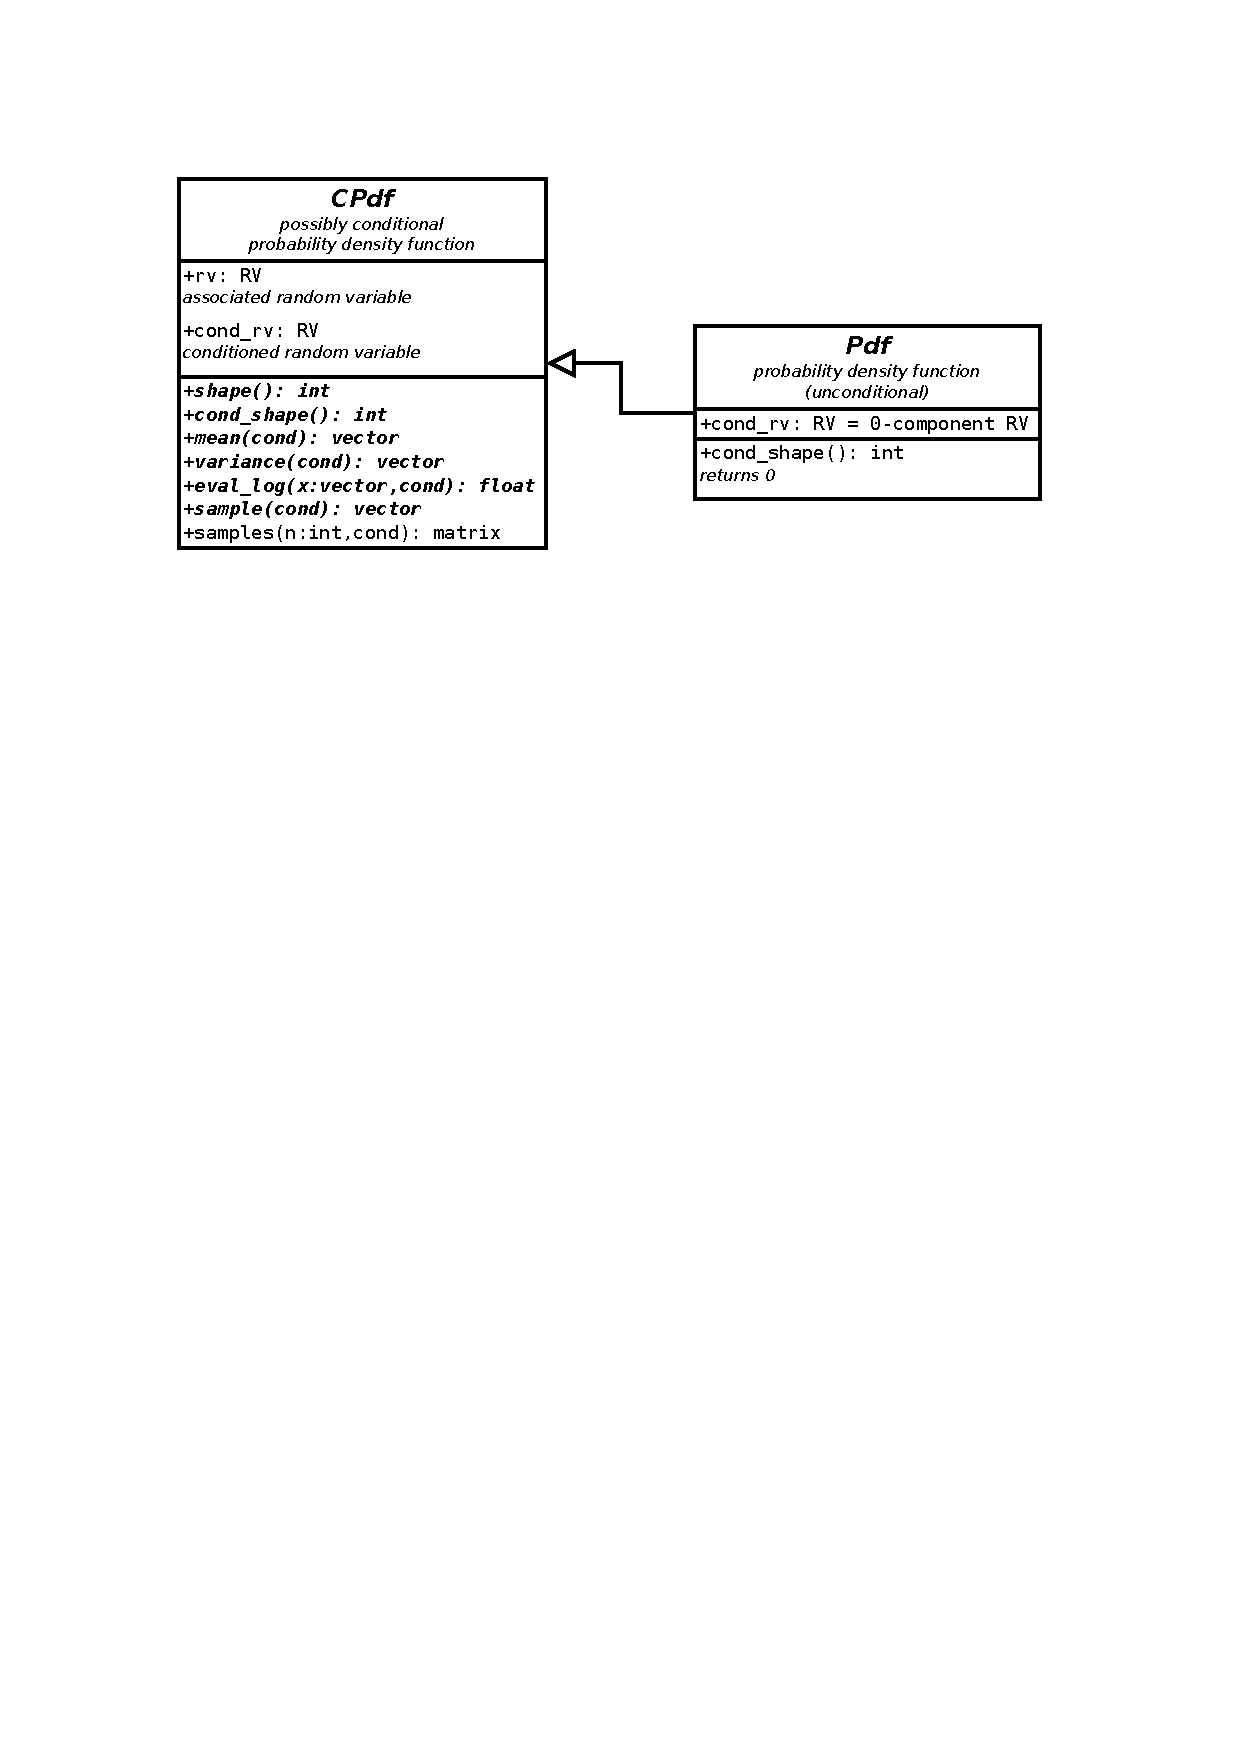
\includegraphics[width=\textwidth,keepaspectratio=true,clip=true,trim=3cm 204mm 3cm 3cm]{./diagrams/pdfs.pdf}
	\vspace{-8mm}
	\caption{Class diagram of the {\pdf} prototypes}
	\label{fig:DiaPdfs}
\end{figure}

The \emph{Pdf} is a very thin subclass of CPdf providing an implementation of the \verb|cond_shape()|
that returns zero to signify empty condition; by convention, Pdf subclasses also should set
\verb|cond_rv| to ``empty random variable''. The function of the Pdf class is therefore rather
semantic than technical distinction between conditional and unconditional {\pdfs}.

Outline of {\pdf} prototypes is shown in the \autoref{fig:DiaPdfs}.

\subsection{Random Variable Meta-representation}

In mathematics, the relation between random variables and {\pdfs} is follows: a {\pdf} is associated
to a random variable, e.g. ``random variable \(X\) is normally distributed''. This is impractical in
software (should drawing a million bare samples produce a million copies of a random variable?) but
let us show that the relation between random variables and {\pdfs} couldn't be entirely dropped
without a substitution, let's look at that following example.

The chain rule for {\pdfs} is heavily used in Bayesian filtering and should be adequately supported
by software. While simple cases can be represented without problems, when for example
\(p(\mathbf{a},\mathbf{b}|\mathbf{c},\mathbf{d})\)
from \eqref{eq:ProdCPdfExample} is desired to be represented, additional information have to be
supplied by the user (programmer) so that the implementation ``knows'' how and what parts of involved
vectors are passed to underlying densities \(p_1\) and \(p_2\). The implementation wouldn't be able
to guess evaluation order, order of components in \(p_1\) condition etc. without such additional
information.
\begin{align}
	p(\mathbf{a},\mathbf{b}|\mathbf{c},\mathbf{d}) &=
		p_1(\mathbf{a}|\mathbf{c},\mathbf{b}) p_2(\mathbf{b}|\mathbf{d}) \label{eq:ProdCPdfExample} \\
	\mathbf{z} &= (\mathbf{a}, \mathbf{b}, \mathbf{c}, \mathbf{d}) =
		(a_1, a_2, b_1, b_2, c_1, c_2, d_1, d_2)  \label{eq:ProdCPdfCombinedVec}
\end{align}

In software it is practical to combine both random and conditioning variable
of the left hand side of \eqref{eq:ProdCPdfExample} into one vector; let \(\mathbf{z}\)
\eqref{eq:ProdCPdfCombinedVec} denote such vector (\(\mathbf{a}, \mathbf{b}, \mathbf{c}, \mathbf{d}\)
are thus all two-dimensional). Now suppose that
the implementation has to pass the vector representing condition \((\mathbf{c}, \mathbf{b})\) to
the distribution \(p_1\) assuming that \(p_2\) was already evaluated. The problem that the software
must solve therefore reduces to the task of finding indexes of the \((\mathbf{c},\mathbf{b})\)
components within vector \(\mathbf{z}\); the solution is indeed an index vector \((5,6,3,4)\),
assuming one-based indexing.

The first option of passing such information from the user to the implementation would be to force
her to specify the relations between distributions manually
using index vectors (or a similar measure) directly; we believe that it is however error-prone
and inconvenient. The other method is to make a symbolic association between {\pdfs} and random
variable descriptions, but the other way around --- {\pdfs} would ``contain'' the description of
random variables they make use of, in our example above \(p_1\) would contain an information
that it is associated with random variable \((\mathbf{a}\)) and conditioning variable
\((\mathbf{c},\mathbf{b})\).

The second approach is used in PyBayes even though it brings some computational overhead (that we
think is worth the simplicity it brings). As mentioned in the previous section, the CPdf class has
\verb|rv| and \verb|cond_rv| attributes that hold instances of the RV class. Simply put, the concept
of random variable meta-representation can be viewed as a kind of \emph{semantic}, or \emph{symbolic
indexing} that should make the life of the PyBayes user easier.

The \emph{RV} class is essentially a list of ``random variable components'' represented using the
RVComp objects. RV provides a few methods to test relationships between 2 random variables
(whether a RV is subset of another RV etc.) and one notable method, \verb|indexed_in()| (that happen
to be shown in the \autoref{fig:Coverage} on page \pageref{fig:Coverage}). Suppose
that RV \(x\) has components \((x_1, x_2, \dotsc, x_n)\) and RV \(y\) is a subset of \(x\) and contains
components \((x_{i_1}, x_{i_2}, \dotsc, x_{i_m})\); \verb|y.indexed_in(x)| then returns an index array
\((i_1, i_2, \dotsc, i_m)\) which is suitable for NumPy array indexing methods.\footnote{the notation
used here is simplified; actual implementation allows for multivariate components \(x_i\) --- \(i_j\)
in returned index array are therefore ranges of integers.}

The \emph{RVComp} class is a simple container for the \verb|dimension| (which must be greater than
zero) and \verb|name| (which is optional) attributes; RV caches aggregate name and dimension. An
important principle in PyBayes is that RVComp comparisons are \emph{instance-based}: 2 RVComp
objects are considered equal if and only if they refer to the same instance.\footnote{the name
attribute thus serves only for aesthetic purposes.} This is fast (compared to for example
name-based equality), saves memory, prevents collisions and is convenient in Python thanks to its
call-by-object semantics. The effects are best demonstrated in the following recording of an
interactive Python session:

\begin{Verbatim}[samepage=true,gobble=1,label=RV and RVComp demonstration,frame=single]
	>>> rv = RV(RVComp(1, "a"))
	>>> rv.contains(RVComp(1, "a"))
	False

	>>> a = RVComp(1, "pretty name")
	>>> b = RVComp(1, "pretty name")  # same name, different instance
	>>> rv = RV(a)
	>>> rv.contains(a)
	True
	>>> rv.contains(b)
	False
\end{Verbatim}
A RVComp without a name (with \verb|name| attribute set to None), that can be called \emph{anonymous
component}, is created in CPdf when the user doesn't pass RV to the constructor, but is otherwise
insignificant.

\begin{figure}[ht]
	\centering
	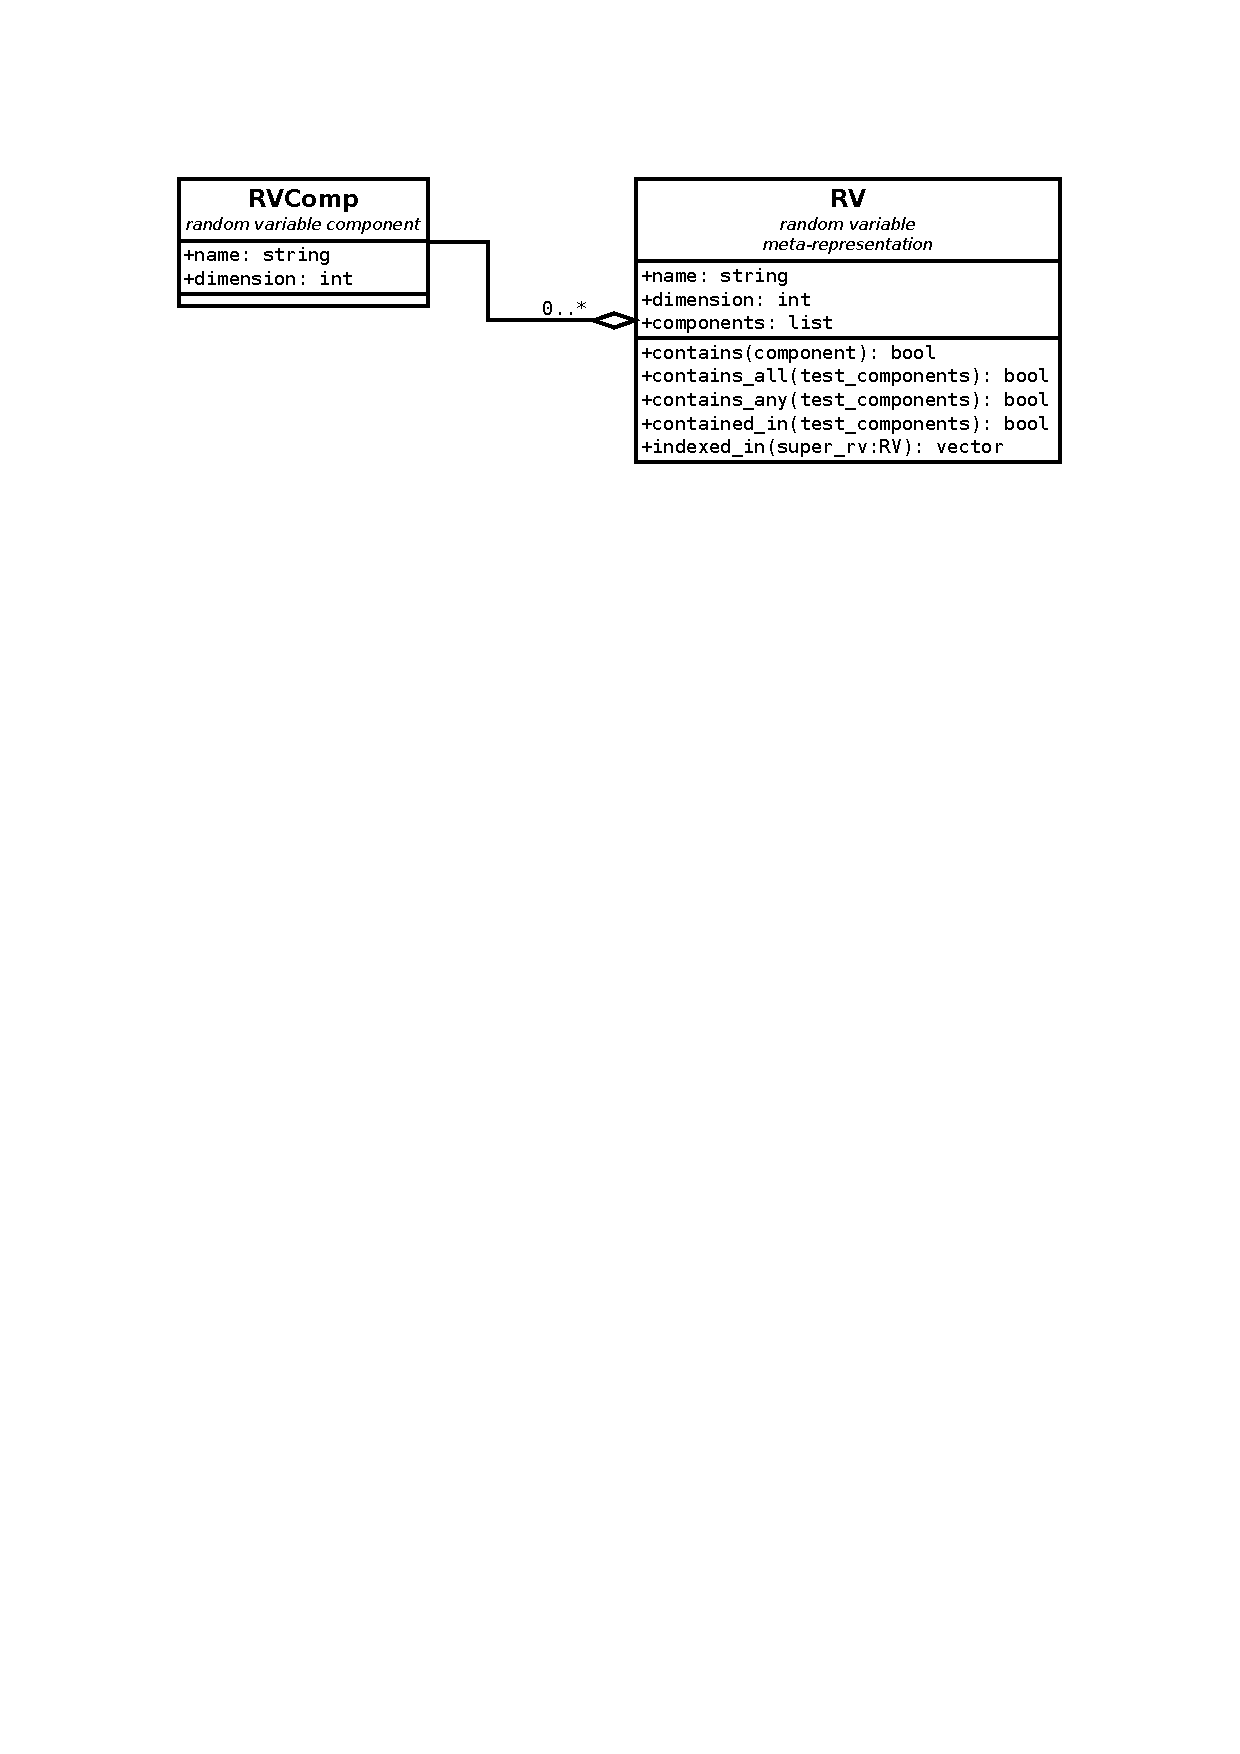
\includegraphics[width=\textwidth,keepaspectratio=true,clip=true,trim=3cm 218mm 3cm 3cm]{./diagrams/rvs.pdf}
	\vspace{-8mm}
	\caption{Class diagram of the random variable framework}
	\label{fig:DiaRvs}
\end{figure}

The concept of random variables might be used also for some Bayesian filters in future should there
be a need for it. On the other hand, documented conventions (such as ordering of vector components)
are used rather than RVs where feasible. Overview of RV and RVComp classes can be seen in the
\autoref{fig:DiaRvs}.

\subsection{Gaussian Probability Density Functions}

We continue by a brief mention of implemented {\pdfs}; our policy is to add new distributions on
as-needed basis rather than trying to have exhaustive set from the beginning. Every user of
PyBayes can create its own distributions by subclassing Pdf of CPdf and implementing meaningful
methods (there is no requirement for implementing unused methods).

PyBayes ships standard multivariate normal (Gaussian) {\pdf} through the \emph{GaussPdf} class;
related log-normal {\pdf} \emph{LogNormPdf} is also provided and shares common abstract superclass,
\emph{AbstractGaussPdf} with GaussPdf. The AbstractGaussPdf class only holds mean attribute \verb|mu|
and covariance matrix attribute \verb|R| and is useful mainly for the family of conditional Gaussian
{\pdfs} described below.

The most general conditional Gaussian distribution is the \emph{GaussCPdf} class that takes two
functions \verb|f| and \verb|g| as parameters\footnote{currently any Python callable objects are
accepted; NumPy \verb|ufunc| class will be evaluated for suitability in future.}
plus the optional \verb|base_class| parameter in
constructor. The \verb|base_class| parameter defaults to GaussPdf, but can be set tu LogNormPdf (to
any AbstractGaussPdf subclass in general); the base class parameter determines resulting density ---
both conditional normal and log-normal distributions can be obtained without any code duplication,
thanks to abstraction provided by AbstractGaussPdf. GaussPdf transforms supplied condition \(c\)
using \eqref{eq:GaussCPdf}, substitutes to AbstractGaussPdf and calls respective \verb|base_class|
method.
\begin{equation} \label{eq:GaussCPdf}
	\begin{aligned}
		\mu &= f(c) \\
		R &= g(c)
	\end{aligned}
\end{equation}

First specialisation of GaussCPdf is the \emph{LinGaussCPdf} class that assumes that \verb|f| and
\verb|g| functions are linear, the transformation is thus according to \eqref{eq:LinGaussCPdf} where
condition is divided into parts \((c_1, c_2)\). The \verb|A|, \verb|C| (matrices), \verb|b| and
\verb|d| (vector) parameters are passed to the constructor. LinGaussCPdf exists mainly for
performance reasons and slightly higher convenience when passing arrays compared to functions;
LinGaussCPdf also benefits from generalisation offered AbstractGaussPdf.
\begin{equation} \label{eq:LinGaussCPdf}
	\begin{aligned}
		\mu &= A c_1 + b \\
		R &= C c_2 + d
	\end{aligned}
\end{equation}

The last GaussCPdf specialisation is the MLinGaussCPdf class which works almost identically as
LinGaussCPdf with the exception that the \verb|R| (covariance) parameter is fixed. Transformation
used by MLinGaussCPdf is thus defined by \eqref{eq:MLinGaussCPdf} where \(c\) is the conditioning
variable. MLinGaussCPdf also supports setting \verb|base_class| as usual.
\begin{equation} \label{eq:MLinGaussCPdf}
	\mu = A c + b
\end{equation}

See the \autoref{fig:DiaGaussPdfs} for a survey of Gaussian and related {\pdfs}.

\begin{figure}[h]
	\centering
	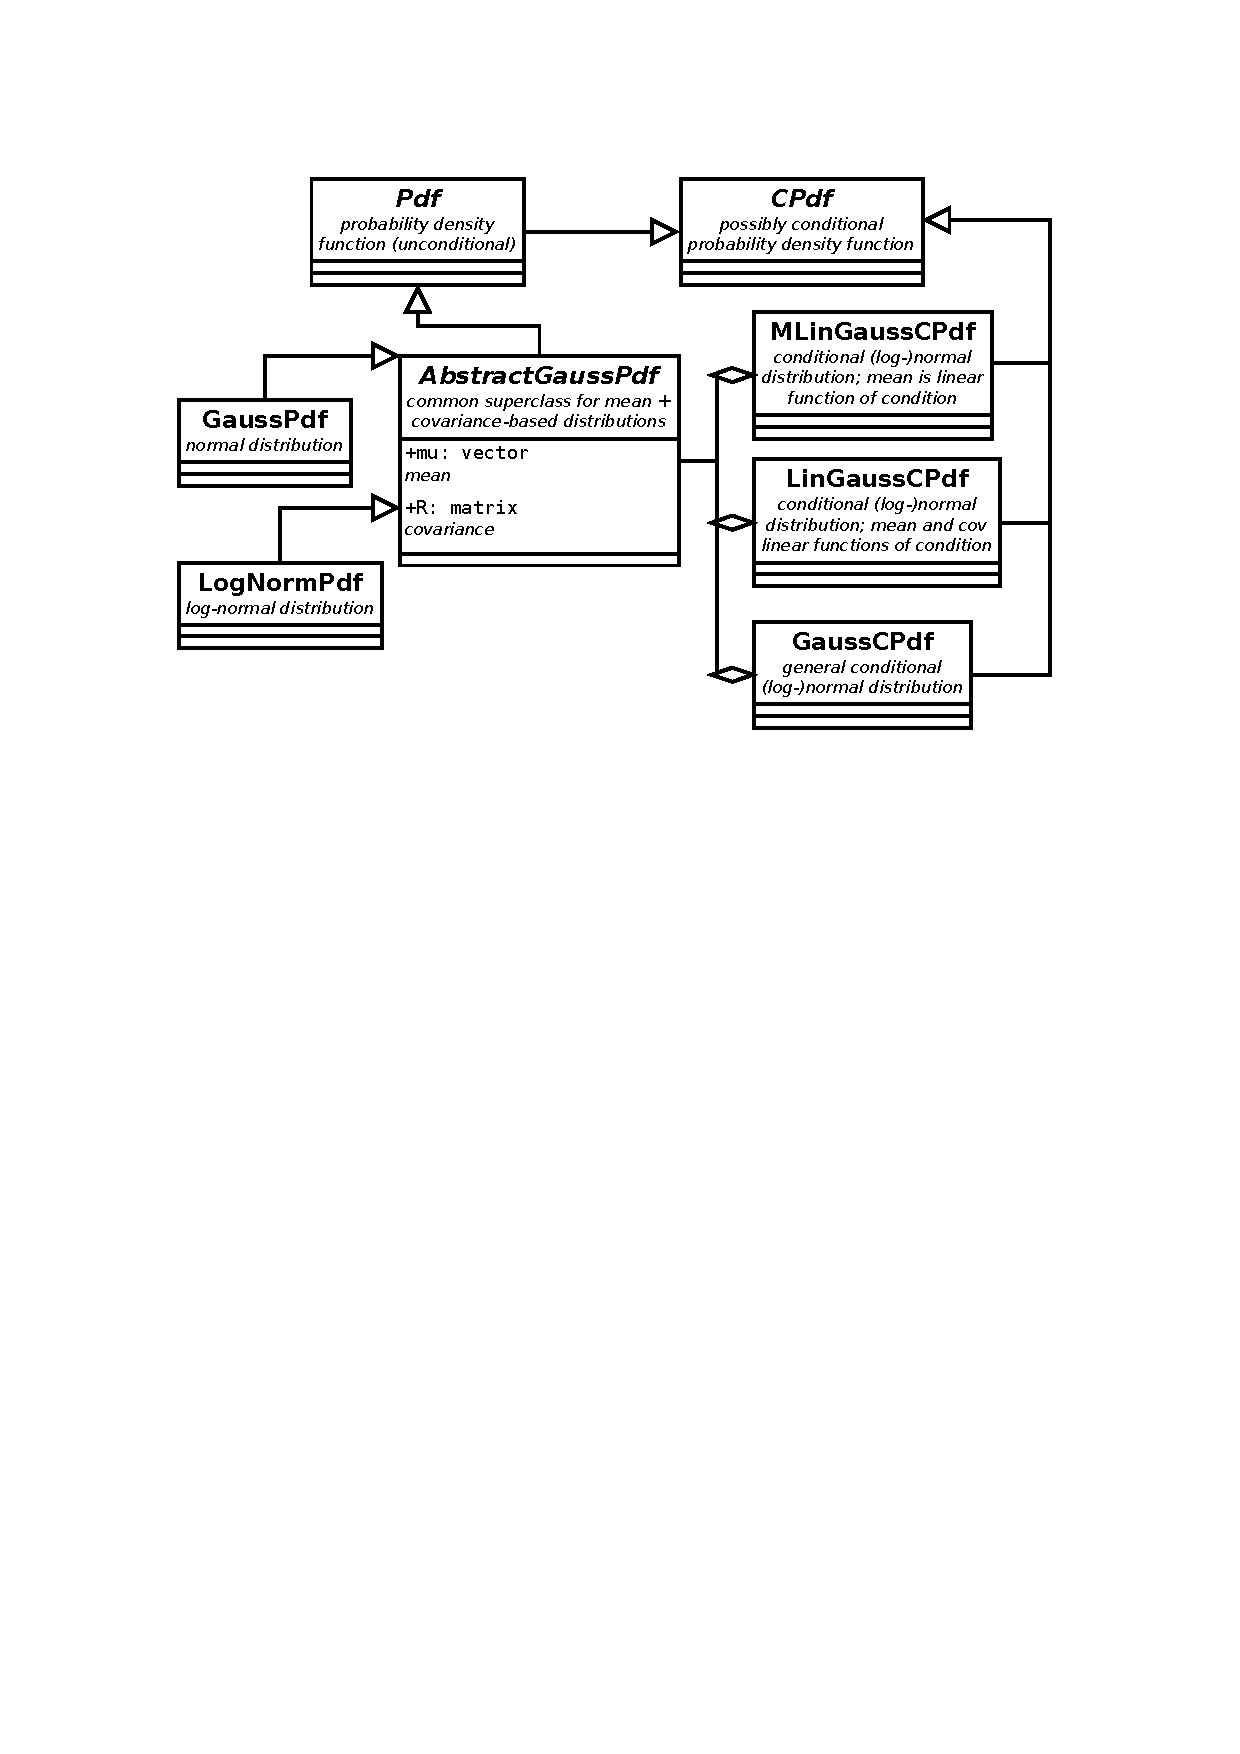
\includegraphics[width=\textwidth,keepaspectratio=true,clip=true,trim=3cm 173mm 3cm 3cm]{./diagrams/gaussian_pdfs.pdf}
	\vspace{-8mm}
	\caption{Class diagram of Gaussian and related distributions}
	\label{fig:DiaGaussPdfs}
\end{figure}

\subsection{Empirical Probability Density Functions}

Another very useful set of distributions is the empirical family suitable for particle filters.
Weighted empirical distribution named EmpPdf in PyBayes is the posterior {\pdf} of the
particle filter while a special product of weighted empirical distribution and a mixture of Gaussian
distributions is the posterior {\pdf} of the marginalized particle filter and is thus named
MarginalizedEmpPdf. Both inherit from AbstractEmpPdf in order to reuse code. Neither of the empirical
densities implement \verb|eval_log()| or \verb|sample()| --- while the latter would be possible, we
are yet to find a valid use-case for it (resampling particles being implemented differently).

The \emph{AbstractEmpPdf} class holds the \verb|weights| parameter, a vector of particle weights denoted as
\(\omega = (\omega_1, \omega_2, \dotsc, \omega_n)\) in formulas. The usual constraints
\eqref{eq:AbstractEmpPdfConstraints} must hold. A simple method \verb|normalise_weights()| normalises
weights according to \eqref{eq:AbstractEmpPdfNormalise}.
\begin{align}
	\omega_i >= 0 \quad \forall i \quad \quad & \quad \quad \sum_{i=1}^n \omega_i = 1 \label{eq:AbstractEmpPdfConstraints} \\
	\omega_i' &= \frac{\omega_i}{\sum_{i=1}^n \omega_i} \label{eq:AbstractEmpPdfNormalise}
\end{align}
AbstractEmpPdf provides one more method, \verb|get_resample_indices()| which
(given that there are \(n\) particles) draws \(n\) random samples from itself and returns their
indices. The algorithm is however optimised in a way that only one random sampling is performed; the
results are thus more predictable (or, ``less random''), but this is desired when used for resampling
in particle filters --- its primary (and currently only) use.

The \emph{EmpPdf} class is the standard weighted empirical distribution \eqref{eq:EmpPdf} that extends
AbstractEmpPdf with the \verb|particles| attribute (a matrix) where each row \(x^{(i)}\) represents
one particle. It also provides the \verb|resample()| method that resamples particles using
\verb|get_resample_indices()| and resets weights to be uniformly distributed. EmpPdf has an extra
role in PyBayes, it is used to test \verb|sample()| of other {\pdfs} using the moment method
(sufficient number of samples is generated and sample mean and variance is compared with theoretical
results).
\begin{equation} \label{eq:EmpPdf}
	p(x) = \sum_{i=1}^n \omega_i \delta(x - x^{(i)})
\end{equation}

Related to the empirical density is the \emph{MarginalizedEmpPdf} that exists solely to form the
posterior {\pdf} of the marginalized particle filter. It extends AbstractEmpPdf with a vector of
GaussPdf objects \verb|gausses|, i-th GaussPdf is denoted as \(\mathcal{N}\left(\hat{a}^{(i)},
P^{(i)}\right)\) and a matrix \verb|particles| where i-th row is denoted as \(b^{(i)}\) in
\eqref{eq:MarginalizedEmpPdf}.
\begin{equation} \label{eq:MarginalizedEmpPdf}
	p(a, b) = \sum_{i=1}^n \omega_i \Big[ \mathcal{N}\left(\hat{a}^{(i)}, P^{(i)}\right) \Big]_a
		\delta(b - b^{(i)})
\end{equation}

MarginalizedEmpPdf doesn't provide a method for resampling as this task have to be done in the
particle filter implementation anyway at it has to deal also with the Kalman filters.

The class diagram of empirical {\pdfs} and related is displayed in the \autoref{fig:DiaEmpPdfs}.

\begin{figure}[h]
	\centering
	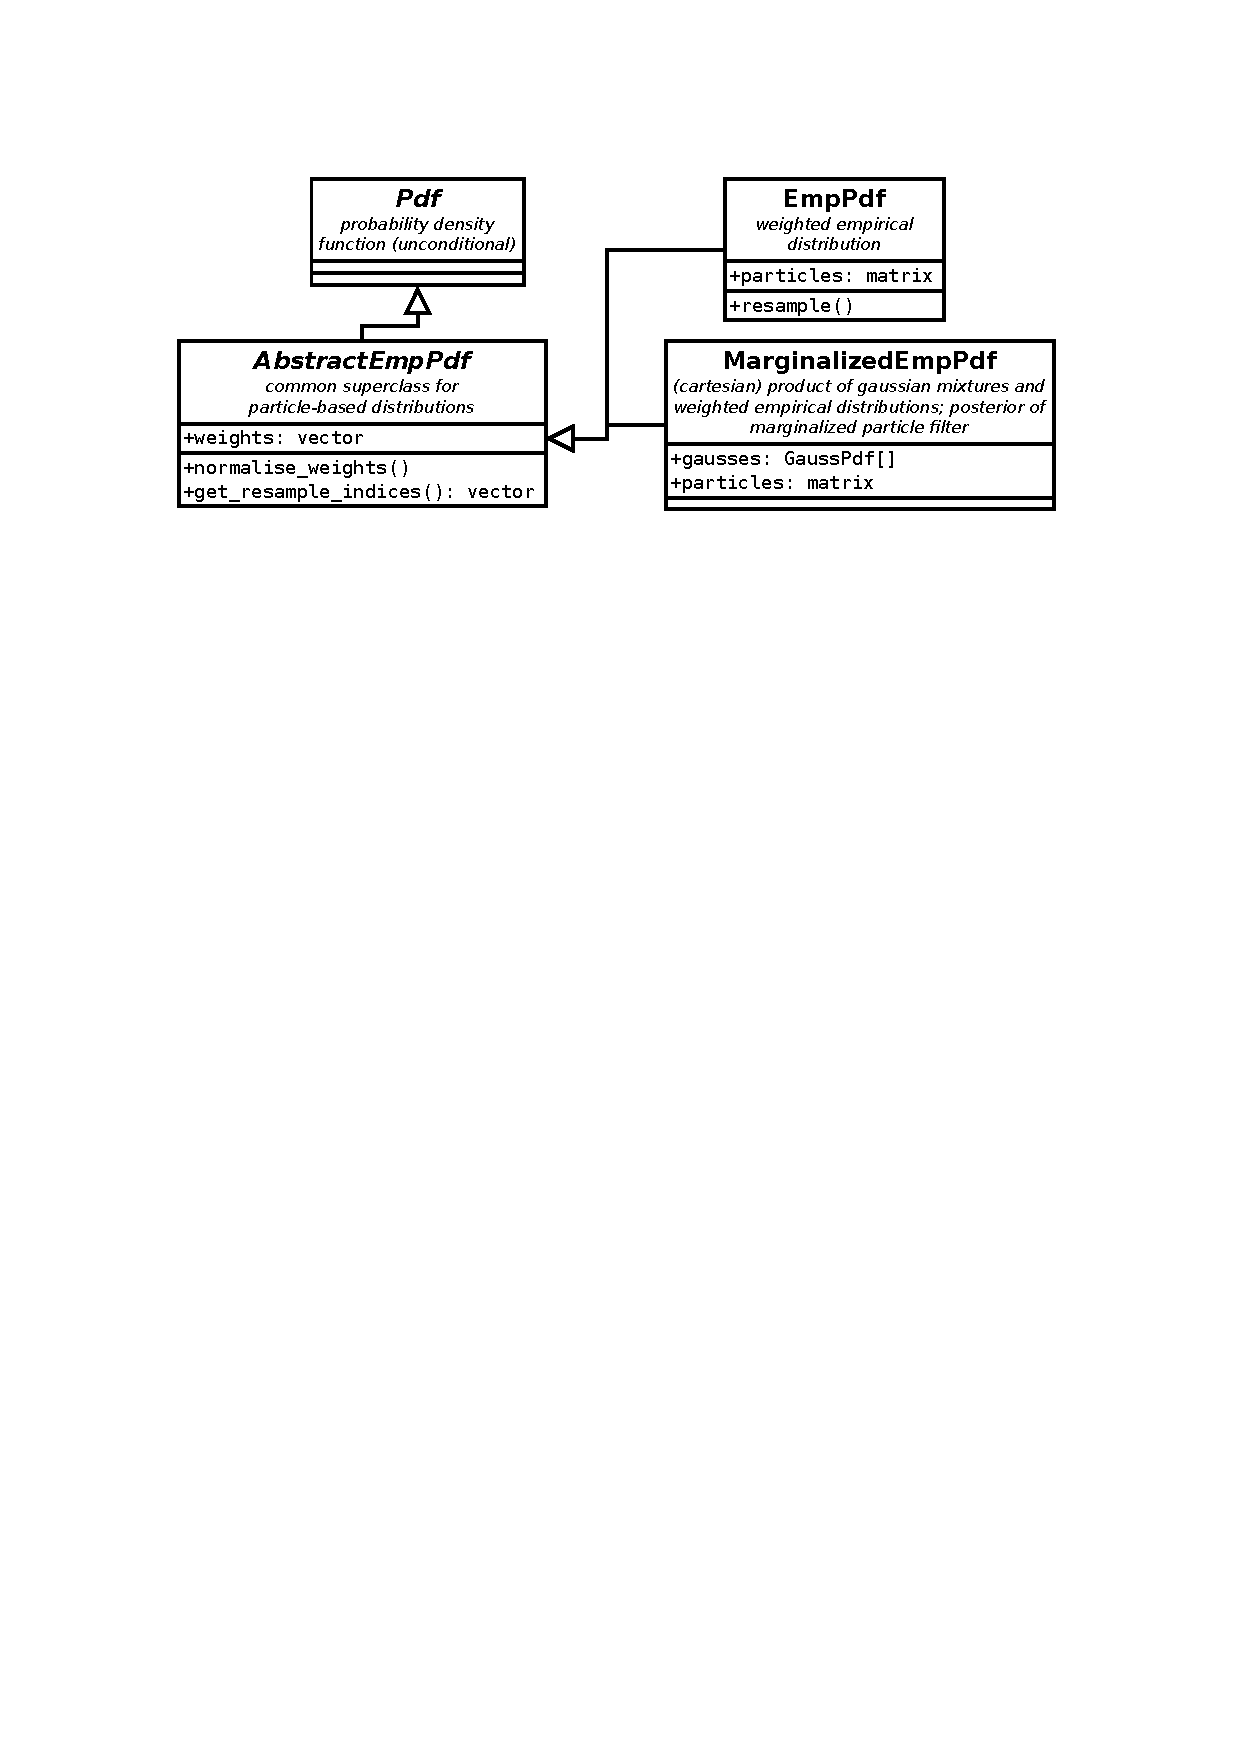
\includegraphics[width=\textwidth,keepaspectratio=true,clip=true,trim=3cm 210mm 3cm 3cm]{./diagrams/emp_pdfs.pdf}
	\vspace{-8mm}
	\caption{Class diagram of empirical distributions}
	\label{fig:DiaEmpPdfs}
\end{figure}

\subsection{Other Probability Density Functions}

We conclude the discussion about the implemented {\pdfs} with the ones that don't fit elsewhere.

The \emph{ProdPdf} class represents unconditional product of \(n\) independent random variables
\(x_1, x_2, \dotsc, x_n\) as depicted in \eqref{eq:ProdPdf}. As an exception from the general rule,
ProdPdf constructs its random variable association (the \verb|rv| attribute) using factor random
variables for convenience; it however currently doesn't make any use of the random variable
meta-representation as it would be of limited usability --- only permutation of random variable
components within \(x_i ~ (\forall i)\) would be additionally possible (the order of factors is
already specified by the user. ProdPdf implements all abstract methods of Pdf by delegating work to
factor {\pdfs}.
\begin{equation} \label{eq:ProdPdf}
	p(x_1, x_2, \dotsc, x_n) = p_1(x_1) p_2(x_2) \dotsm p_n(x_n)
\end{equation}

A more sophisticated variant of the ProdPdf is the \emph{ProdCPdf} class that is potentially
conditional and allows for conditionally dependent random variables. In general it can represent
a~chain rule for
{\pdfs} shown in \eqref{eq:ProdCPdf} with an additional constraint that the right hand side makes
sense (that means that there exists a sequence \((p_{j_1}, p_{j_2}, \dotsc, p_{j_m})\) for which
\eqref{eq:ProdCPdfContraint} holds). The relation ``\(C \subset \{x_i, x_j, x_k, \dotsc\}\)'' denotes
``random variable \(C\) is composed of the (subset of) \(x_i, x_j, x_k, \dotsc\) random variable components''
in the following formulas.
\begin{gather} \label{eq:ProdCPdf}
	\begin{gathered}
		p(x_1, x_2, \dotsc, x_m | x_{m+1}, x_{m+2} , \dotsc, x_n) = p_1(x_1 | C_1)
			p_2(x_2 | C_1) \dotsm p_m(x_m | C_m) \\
		\text{where} \quad m \leq n; \quad
			\forall i \in \{1, 2, \dotsc, m\}: C_i \subset \{x_1, x_2, \dotsc, x_n\}
	\end{gathered}
\end{gather}
\begin{equation} \label{eq:ProdCPdfContraint}
	\forall k \in \{1, 2, \dotsc, m\}: C_{j_k} \subset \{x_1, x_2, \dotsc, x_{k-1}\} \cup \{x_{m+1}, x_{m+2} , \dotsc, x_n\}
\end{equation}

As in ProdPdf, all abstract methods of CPdf are implemented.
ProdCPdf makes extensive use of the random variable meta-representation described earlier; it uses
random variable descriptions of factor densities \(p_1, p_2, \dotsc, p_m\) to construct the
data-flow (the \((p_{j_1}, p_{j_2}, \dotsc, p_{j_m})\) sequence); the order of passed factor
distributions is therefore insignificant --- ProdCPdf always computes correct evaluation order if
it exists. For this reason the random variable components of factor {\pdfs} need to be specified
(at least those that are ``shared'' between multiple factor distributions). Currently, there is also
a limitation that compound random variable representations have to be additionally passed to ProdCPdf;
in future, ProdCPdf will be able to infer compound random variables from factor distributions.
Following code example constructs a simple {\pdf} from \eqref{eq:ProdCPdfSimple}:
\begin{equation} \label{eq:ProdCPdfSimple}
	p(a,b) = p_1(a|b) p_2(b)
\end{equation}

\begin{Verbatim}[samepage=true,gobble=1,label=ProdCPdf example,frame=single]
	# prepare random variables:
	a, b = RVComp(m, "name of a"), RVComp(n, "b name")
	p_1 = SomeCPdf(..., rv=RV(a), cond_rv=RV(b))
	p_2 = OtherPdf(..., rv=RV(b))
	p = ProdCPdf((p_1, p_2), rv=RV(a, b), cond_rv=RV()) # empty cond_rv

	# version 0.4 of PyBayes will allow:
	p = ProdCPdf((p_1, p_2))
\end{Verbatim}
PyBayes also provides a multivariate uniform distribution implemented by the \emph{UniPdf} class.

\subsection{Bayesian Filters}

Bayesian filters are the \emph{raison d'être} of PyBayes. It turned out however that with a solid
framework of {\pdfs}, their implementation is rather straightforward. All filters in PyBayes extend
an abstract class \emph{Filter} that acts as a prototype of all filters. Filter defines following
methods that can/should be implemented by subclasses:
\begin{itemize}
	\item \verb|bayes(yt : vector, cond : vector = None)| \\
		compute posterior {\pdf} given
		the observation \verb|yt|; semantics of the optional \verb|cond| parameter are defined
		by filter implementations. The method name comes from the fact that computing the posterior
		{\pdf} involves applying (exact or approximate) Bayes rule; see \eqref{eq:PosteriorPdfRaw}
		on page \pageref{eq:PosteriorPdfRaw}.
	\item \verb|posterior() : Pdf| \\
		return a reference to the posterior {\pdf} \(p(x_t | y_{1:t})\) \eqref{eq:PosteriorPdf}
		(p.~\pageref{eq:PosteriorPdf}).
	\item \verb|evidence_log(yt : vector) : float| \\
		return logarithm of the marginal likelihood \(p(y_t | y_{1:t-1})\) \eqref{eq:MargLikelihood}
		(p.~\pageref{eq:MargLikelihood}) evaluated in point \verb|yt|. Subclasses may choose not to
		implement this method if it is not feasible.
\end{itemize}
Fists subclass of Filter is the \emph{KalmanFilter} class that implements slightly extended version
of the Kalman filter presented in the first chapter --- KalmanFilter can optionally accept control
vector in its \verb|bayes| method (passed through the \verb|cond| parameter) making it suitable also
for the theory of Bayesian decision-making.

Speaking about the particle filter family, it has been suggested in \cite{Smi:10} that the particle
filter and the marginalized particle filter can be merged into one general class using a recursive
structure of classes representing the Bayes rule (e.g. Filter in PyBayes). This approach has not
been used in PyBayes for performance and simplicity reasons. On the other hand, particle filters in
PyBayes offload much work to {\pdfs} in PyBayes where code is reused thanks to AbstractEmpPdf.

The \emph{ParticleFilter} class implements a simple version of the particle filter as presented in
the first chapter. ParticleFilter takes the process model \(p(x_t|x_{t-1})\) and the observation
model \(p(y_t|x_t)\) distributions in constructor (along with the initial density and number of
particles) and employs \verb|resample()| and \verb|normalise_weights()| of the EmpPdf class that it
uses for the posterior distribution. ParticleFilter currently doesn't support specifying the
proposal density, although it is planned in future.

\emph{MarginalizedParticleFilter} also implements the respective algorithm shown in the first
chapter and offloads some work to its posterior {\pdf}, MarginalizedEmpPdf, but has to provide its
own array of KalmanFilter objects. The MarginalizedParticleFilter class ensures that the i-th Kalman
filter shares its posterior Gaussian distribution with MarginalizedEmpPdf's i-th particle. This is
the reason why resampling cannot be done in MarginalizedEmpPdf and is instead performed in the
\verb|_resample()| method of MarginalizedParticleFilter that makes use of the
\verb|get_resample_indices()| method of AbstractEmpPdf.

In constructor MarginalizedEmpPdf accepts initial distribution of the state vector
\(p(x_0) = p(a_0, b_0)\), process model of the empirical part of the state vector \(p(b_t|b_{t-1})\),
the class of the desired Kalman filter implementation (that has to be a subclass of KalmanFilter)
and its parameters in form of a Python dictionary. That way, thanks to Python capabilities,
MarginalizedEmpPdf will support other variants of the Kalman filter in future without a need to be
changed. It also means that the observation model is specified using the Kalman filter implementation
and parameters for it, which makes MarginalizedParticleFilter more flexible. The process model is
given by the combination of \(p(b_t|b_{t-1})\) and supplied Kalman filter implementation (and its
parameters). Current implementation hard-codes \(b_t\) to be the observation and process noise of
the modelled system; this silly limitation will be lifted in future where MarginalizedParticleFilter
will pass the \(b_t\) vector as the \verb|cond| argument to the \verb|bayes()| method of the
specified Kalman filter implementation.

A diagram of filtering classes in shown in the \autoref{fig:DiaFilters}.

\begin{figure}[h]
	\centering
	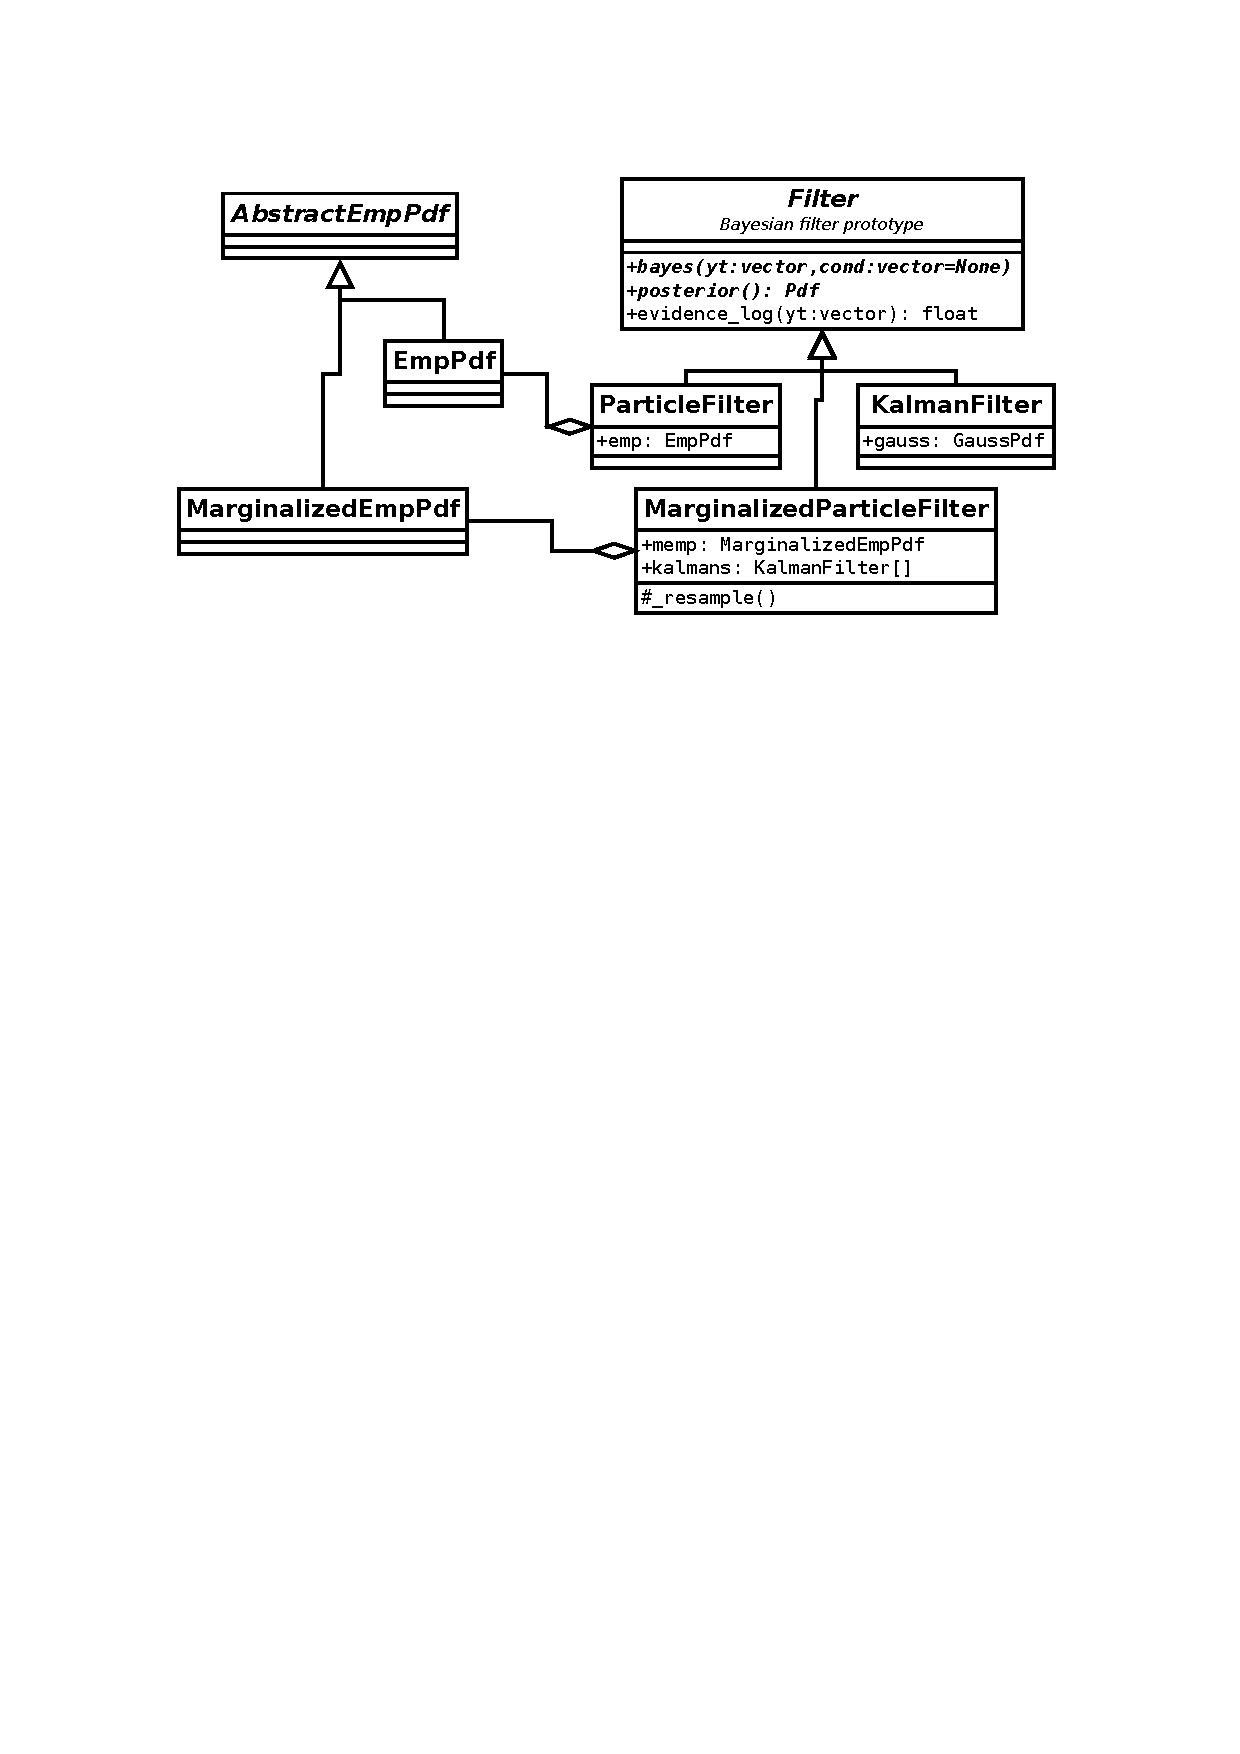
\includegraphics[width=\textwidth,keepaspectratio=true,clip=true,trim=3cm 192mm 3cm 3cm]{./diagrams/filters.pdf}
	\vspace{-8mm}
	\caption{Class diagram of Bayesian filters}
	\label{fig:DiaFilters}
\end{figure}

\subsection{Wrappers} \label{sec:PyBayesWrappers}

Favourable performance was one of the criteria for the desired library for Bayesian filtering. When
the performance of the KalmanFilter class was benchmarked with a small system (both state and
observation vectors were 2-dimensional); it was discovered that a great portion of total run time
was spent in the boilerplate code of NumPy functions \verb|dot()| (for matrix product) and
\verb|inv()| (for matrix inversion). Even though NumPy uses BLAS and LAPACK internally, the time
spent in the intermediate Python code was unacceptable (it was probably made more visible due to
the small size of the system); see the \autoref{sec:CythonFeatures} on page
\pageref{sec:CythonFeatures} for information about Cython \(\leftrightarrow \) NumPy co-operation.

Fortunately, a project that approaches popular BLAS and LAPACK functions more directly was found:
Shane Legg's Tokyo\footnote{\url{http://www.vetta.org/2009/09/tokyo-a-cython-blas-wrapper-for-fast-matrix-math/}}
wraps BLAS (and a couple of LAPACK) procedures in Cython using NumPy's \verb|ndarray| data-type.
Quick tests have shown great speed-ups --- the mentioned functions ceased to be performance
bottle-necks. It was therefore decided that the Tokyo project should be used in the Cython mode of
PyBayes and it was forked\footnote{\url{https://github.com/strohel/Tokyo}} on github to provide
a~couple of bug-fixes we made to the public. For convenience, Tokyo is also bundled with PyBayes
releases and is built along it to reduce dependencies on obscure libraries.

A special approach in PyBayes has been taken in order to support both Python and
Cython mode: wrapper modules for \verb|numpy| and \verb|numpy.linalg| were created in the
\verb|pybayes.wrappers| package; Python versions of the wrappers (.py files) just import appropriate
NumPy modules. Cython versions do nearly the same, but provide own implementations (that call Tokyo)
of the offending NumPy functions (and delegate the rest to NumPy). Other code then imports
\verb|wrappers._numpy| instead of \verb|numpy|, likewise for \verb|numpy.linalg|.

\section{Documentation and Testing} \label{sec:PyBayesDocsTests}

Second pillar of each well-written software library is, in our belief, its \emph{documentation}; the
first one being the library design and the actual implementation being no better than the third
pillar (in our view, the implementation can be easily modified in a well-designed library). PyBayes
reflects that and puts great emphasis on the API Documentation, that is
\ifattachements included in appendix on page \pageref{chap:APIDocs}, on the bundled CD-ROM and \fi
accessible on-line at \url{http://strohel.github.com/PyBayes-doc/}.

Documentation is generated almost solely from the documenting comments --- Python ``Docstrings'' as
defined in PEP 257,\footnote{Python Enhancement Proposal 257: \url{http://www.python.org/dev/peps/pep-0257/}}
using the Sphinx Python documentation generator.\footnote{\url{http://sphinx.pocoo.org/}} Sphinx
supports additional syntax in Docstrings and is able to generate documentation in a wide range of
formats including HTML, Qt Help,\footnote{\url{http://doc.qt.nokia.com/qthelp-framework.html}}
Devhelp,\footnote{\url{http://live.gnome.org/devhelp}} \LaTeX, PDF, man-pages and many others. One
very valuable feature of Sphinx is the ability to parse {\LaTeX}-encoded mathematics embedded
directly into Docstrings; these are then rendered to images in HTML output for example.

Every publicly available class and method in PyBayes is extensively documented and enhanced with
mathematical formulas where appropriate. We believe that this approach makes
PyBayes more easily usable by mathematicians and eliminates any possible misunderstanding of the textual
description of classes and methods. An example of how Docstrings look like in code can be seen in
the \autoref{fig:Coverage}. We must say we are very satisfied with Sphinx can only recommend using
it.

As noted in the discussion about dynamically-typed languages, almost all programmer errors in such
languages are only discovered at runtime, therefore a need for a comprehensive test-suite was
stressed out. PyBayes follows this advice and provides two packages that accomplish testing:
\begin{itemize}
	\item \verb|pybayes.tests| \\
		package contains unit-tests of virtually all PyBayes classes and methods. Unit-testing
		evaluates classes and methods \emph{in isolation} (to highest possible extent) and therefore
		forms an excellent tool for finding precise location of possible bugs. Unit-testing should
		last no longer than a few seconds so that it can be run on per-commit basis. One problem
		faced in PyBayes are non-deterministic methods such as \verb|CPdf.sample()| or
		\verb|bayes()| methods of particle filters. \verb|sample()| methods are currently tested
		by generating high enough number of particles and then comparing their mean and variance
		with theoretical values.
		Another option would be mocking the random number generator to force deterministic results,
		this could however produce false-positives when an implementation of a given \verb|sample()|
		method changed.

		PyBayes currently contains 99 unit-tests that run in approximately 0.2 seconds.
	\item \verb|pybayes.stresses| \\
		package contains so-called stress-tests --- longer-running procedures that test greater
		portion of code and cooperation if individual modules. Results of stresses are not intended
		be checked automatically, they rather require human evaluation. PyBayes currently has three
		stresses, one for each Bayesian filter implementation, that are run with various parameters
		to ensure that the filters produce valid-looking results, to measure their performance, and
		(for particle filters) to test their convergence as the number of particles increases.
\end{itemize}
To ensure that all code-paths are properly tested, it is advisable to employ a \emph{code coverage}
tool that shows which code statements were visited during tests. We've used Ned Batchelder's excellent
\emph{coverage.py}\footnote{\url{http://nedbatchelder.com/code/coverage/}} to discover that 86\%
statements in the \verb|pdfs| module and 83\% statements in the \verb|filters| module are covered
by tests and stress-tests combined. An example output of coverage.py is shown in the
\autoref{fig:Coverage}, where everything except one code-path throwing an exception is covered by
a test.

\begin{figure}[h]
	\centering
	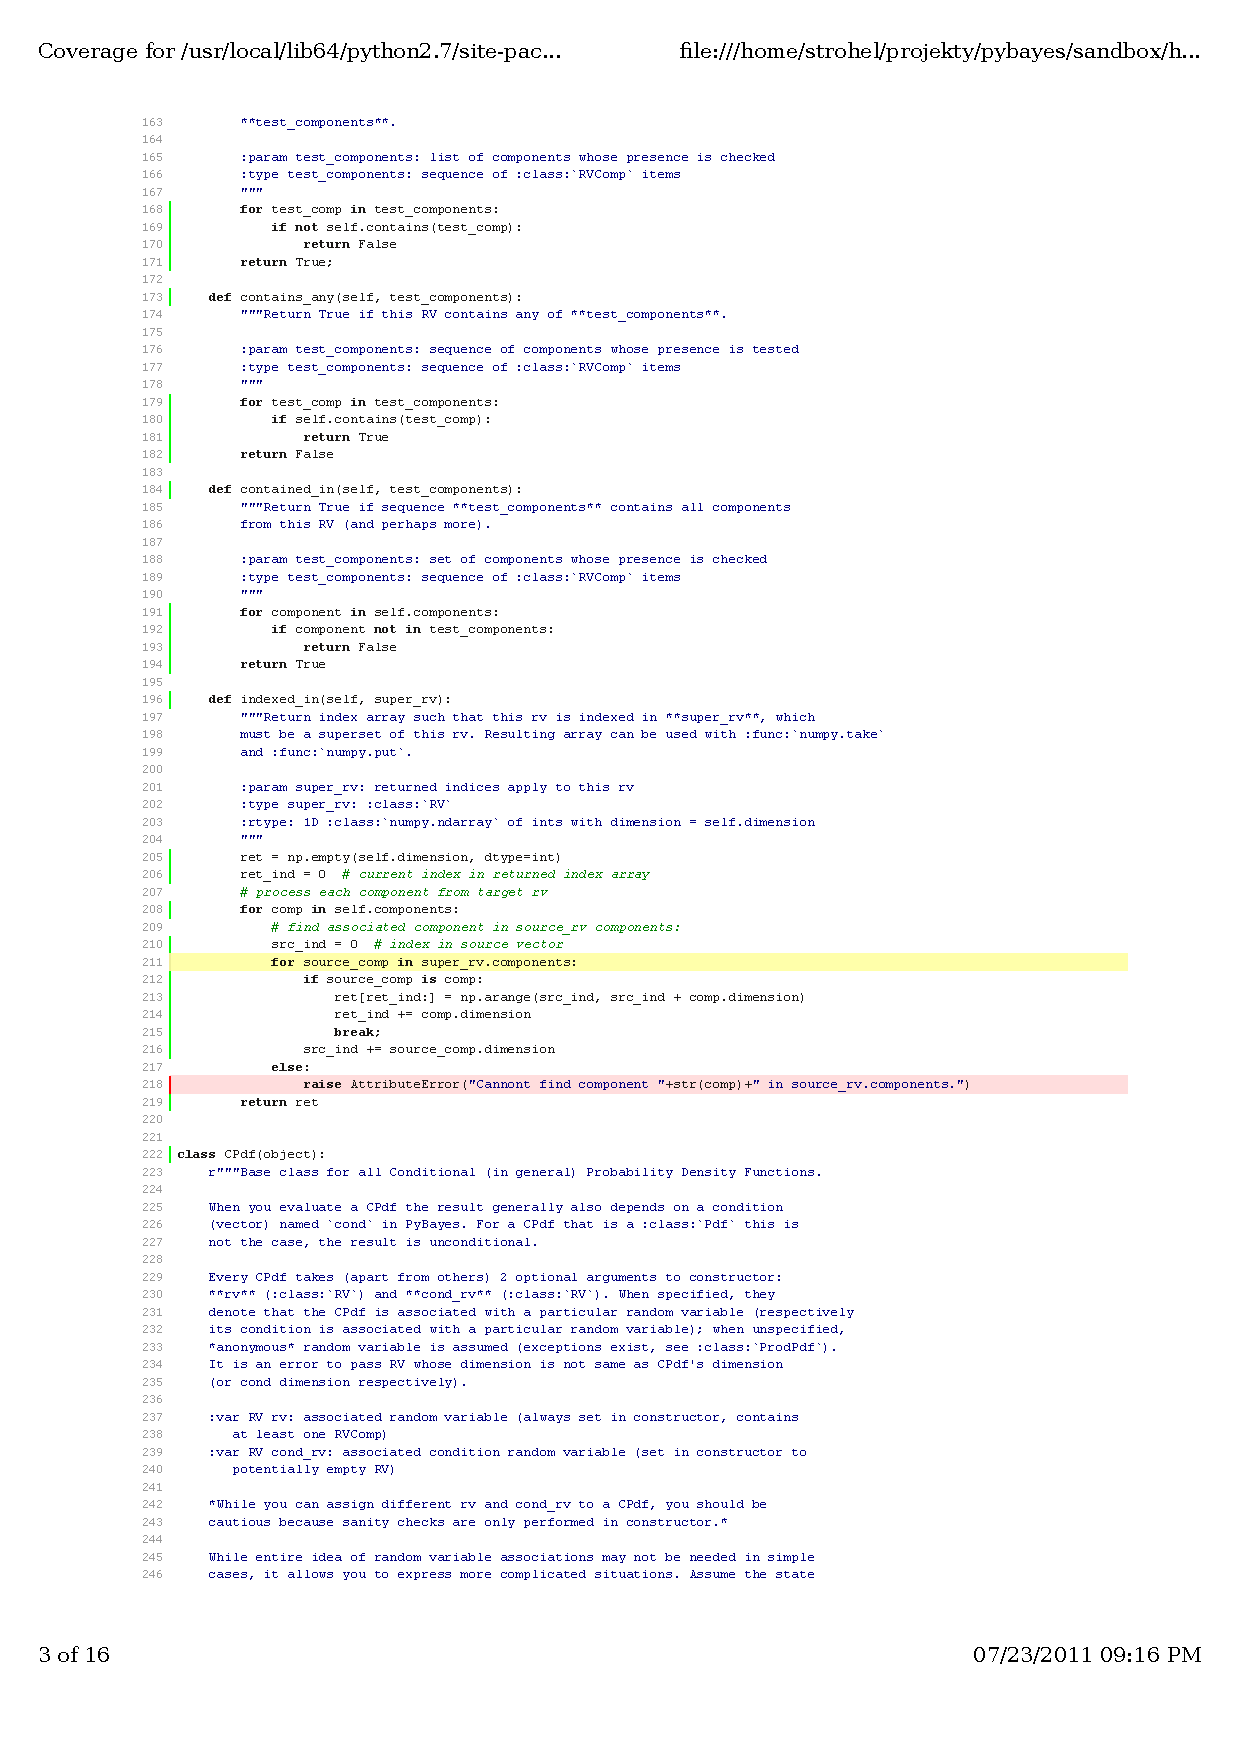
\includegraphics[width=\textwidth,keepaspectratio=true,clip=true,trim=24mm 109mm 60mm 117mm]{./coverage.pdf}
	\vspace{-8mm}
	\caption{coverage.py shows that one code-path in indexed\_in() is uncovered}
	\label{fig:Coverage}
\end{figure}

\section{Performance Comparison with BDM} \label{sec:PyBayesPerformance}

The chapter about the PyBayes library is concluded by a benchmark of four various Kalman filter
implementations from PyBayes and BDM~\cite{BDM}. All tested implementations use exactly the same
algorithm and equivalent data-types, neither is explicitly parallelised (however, see notes about
MATLAB), operate on the same data and gave exactly the same results as shown in the \autoref{fig:KF}
on page \pageref{fig:KF}. Following versions of involved software were used:
\begin{description}
	\item[Python] 2.7.1
	\item[GNU C Compiler] 4.4.5; \verb|-O2| optimisation flag used when compiling C files
	\item[Cython] 0.14.1+ (git revision 0.14.1-1002-g53e4c10)
	\item[MATLAB] 7.11.0.584 (R2010b) 64-bit (glnxa64)
	\vspace{1mm}
	\item[PyBayes] 0.3
	\item[BDM] SVN revision r1378
\end{description}

The test was performed on a 64-bit dual-core Intel Core i5-2520M CPU clocked at 2.50 Ghz with Intel Turbo
Boost and Hyper-threading enabled; operating system is Gentoo Linux compiled for the x86\_64 platform.

The test consists of running 3000 iterations of the Kalman filter with various state-space dimensions:
2, 30 and 60; observation vector is has the same dimensionality as the state vector. Wall-clock time
needed to complete all iterations is measured. Each implementation was tested 10 times, mean values
are shown; to measure variance across runs, relative sample standard deviation \(s_{\text{rel}}\)
computed using \eqref{eq:RelStdDev} (page \pageref{eq:RelStdDev}) was measured. Additionally,
relative speed-up with regards to reference version \textbf{PyBayes Cy} is displayed for
illustration. Following versions of Kalman filter/implementation environments were under test:
\begin{description}
	\item[PyBayes Py] \hfill \\
		KalmanFiler class from PyBayes \url{pybayes/filters.py}; Python build
	\item[PyBayes Cy] \hfill \\
		KalmanFiler class from PyBayes \url{pybayes/filters.py}; Cython build
	\item[MATLAB imper.] \hfill \\
		Imperative MATLAB implementation where the whole algorithm is written
		in a single for loop; comes from BDM, file \url{library/tests/stressuite/kalman_stress.m}.
		While not explicitly parallelised, later experiments shown that MATLAB implicitly
		parallelised the code behind curtain at least in higher-dimensional cases.
	\item[MATLAB o-o] \hfill \\
		Object-oriented MATLAB implementation from BDM where the filter and Gaussian {\pdf} is
		represented using MATLAB classes; file \url{applications/bdmtoolbox/mex/mexKalman.m}.
	\item[BDM] \hfill \\
		 Object-oriented C++ class KalmanFull from BDM implemented in
		 \url{/library/bdm/estim/kalman.cpp}.
\end{description}
Benchmark results are shown in tables \ref{tab:KFSmall} to \ref{tab:KFHuge}. The greatest variance
in results is achieved in the small (2-dimensional) system, where the C++ version is the fastest,
outperforming Cython build of PyBayes by 260\% and object-oriented MATLAB version was embarrassingly
15\x\ slower than the PyBayes Cy.

\begin{table}[h!]
	\centering
	\begin{tabular}{|r|l|l|l|l|l|} \hline
		& PyBayes Py & PyBayes Cy & MATLAB imper. & MATLAB o-o & BDM \\ \hline
		time [s] & 0.254 & 0.091 & 0.069 & 1.378 & 0.026 \\ \hline
		\(s_{\text{rel}}\) & 4.4\% & 4.2\% & 8.5\% & 4.1\% & 9.3\% \\ \hline
		speed-up & 0.4\x & 1.0\x & 1.3\x & 0.1\x & 3.6\x \\ \hline
	\end{tabular}
	\caption{Performance of Kalman filters: 2-dimensional state-space}
	\label{tab:KFSmall}
	\vspace{7mm}

	\begin{tabular}{|r|l|l|l|l|l|} \hline
		& PyBayes Py & PyBayes Cy & MATLAB imper. & MATLAB o-o & BDM \\ \hline
		time [s] & 0.689 & 0.535 & 0.424 & 1.780 & 0.518 \\ \hline
		\(s_{\text{rel}}\) & 3.0\% & 5.4\% & 5.9\% & 2.7\% & 5.7\% \\ \hline
		speed-up & 0.8\x & 1.0\x & 1.3\x & 0.3\x & 1.0\x \\ \hline
	\end{tabular}
	\caption{Performance of Kalman filters: 30-dimensional state-space}
	\label{tab:KFBig}
	\vspace{7mm}

	\begin{tabular}{|r|l|l|l|l|l|} \hline
		& PyBayes Py & PyBayes Cy & MATLAB imper. & MATLAB o-o & BDM \\ \hline
		time [s] & 2.120 & 1.816 & 1.274 & 3.849 & 1.948 \\ \hline
		\(s_{\text{rel}}\) & 2.4\% & 2.6\% & 6.3\% & 9.9\% & 2.1\% \\ \hline
		speed-up & 0.9\x & 1.0\x & 1.4\x & 0.5\x & 0.9\x \\ \hline
	\end{tabular}
	\caption{Performance of Kalman filters: 60-dimensional state-space}
	\label{tab:KFHuge}
\end{table}

Raising the dimensionality of state-space to 30 produced more even results with object-oriented
MATLAB still lagging behind, PyBayes Cy and C++ version from BDM being nearly equal and imperative
MATLAB version taking lead by being approximately 30\% faster.

A huge 60-dimensional system sees PyBayes Py, PyBayes Cy and BDM versions being even closer,
imperative MATLAB version extending its advantage and object-oriented MATLAB version still largely
unusable due to its poor performance.

The chart shown in the \autoref{fig:KFPerf} allows for some speculations about possible reasons
of performance differences. First, it seems that the Python version adds moderate per-statement
overhead that doesn't raise with number of dimensions (we blame NumPy for Python version being
on par with the C++ and Cython versions) while object-oriented MATLAB adds \textbf{enormous} overhead
that worsens slightly with number of dimensions.

The clear advantage of the imperative MATLAB version can be accounted to its capability to parallelise
code behind the scenes, in our belief. Our informal late tests have shown that it performs very
close to the PyBayes Cy version on uniprocessor systems.

\begin{figure}[h]
	\centering
	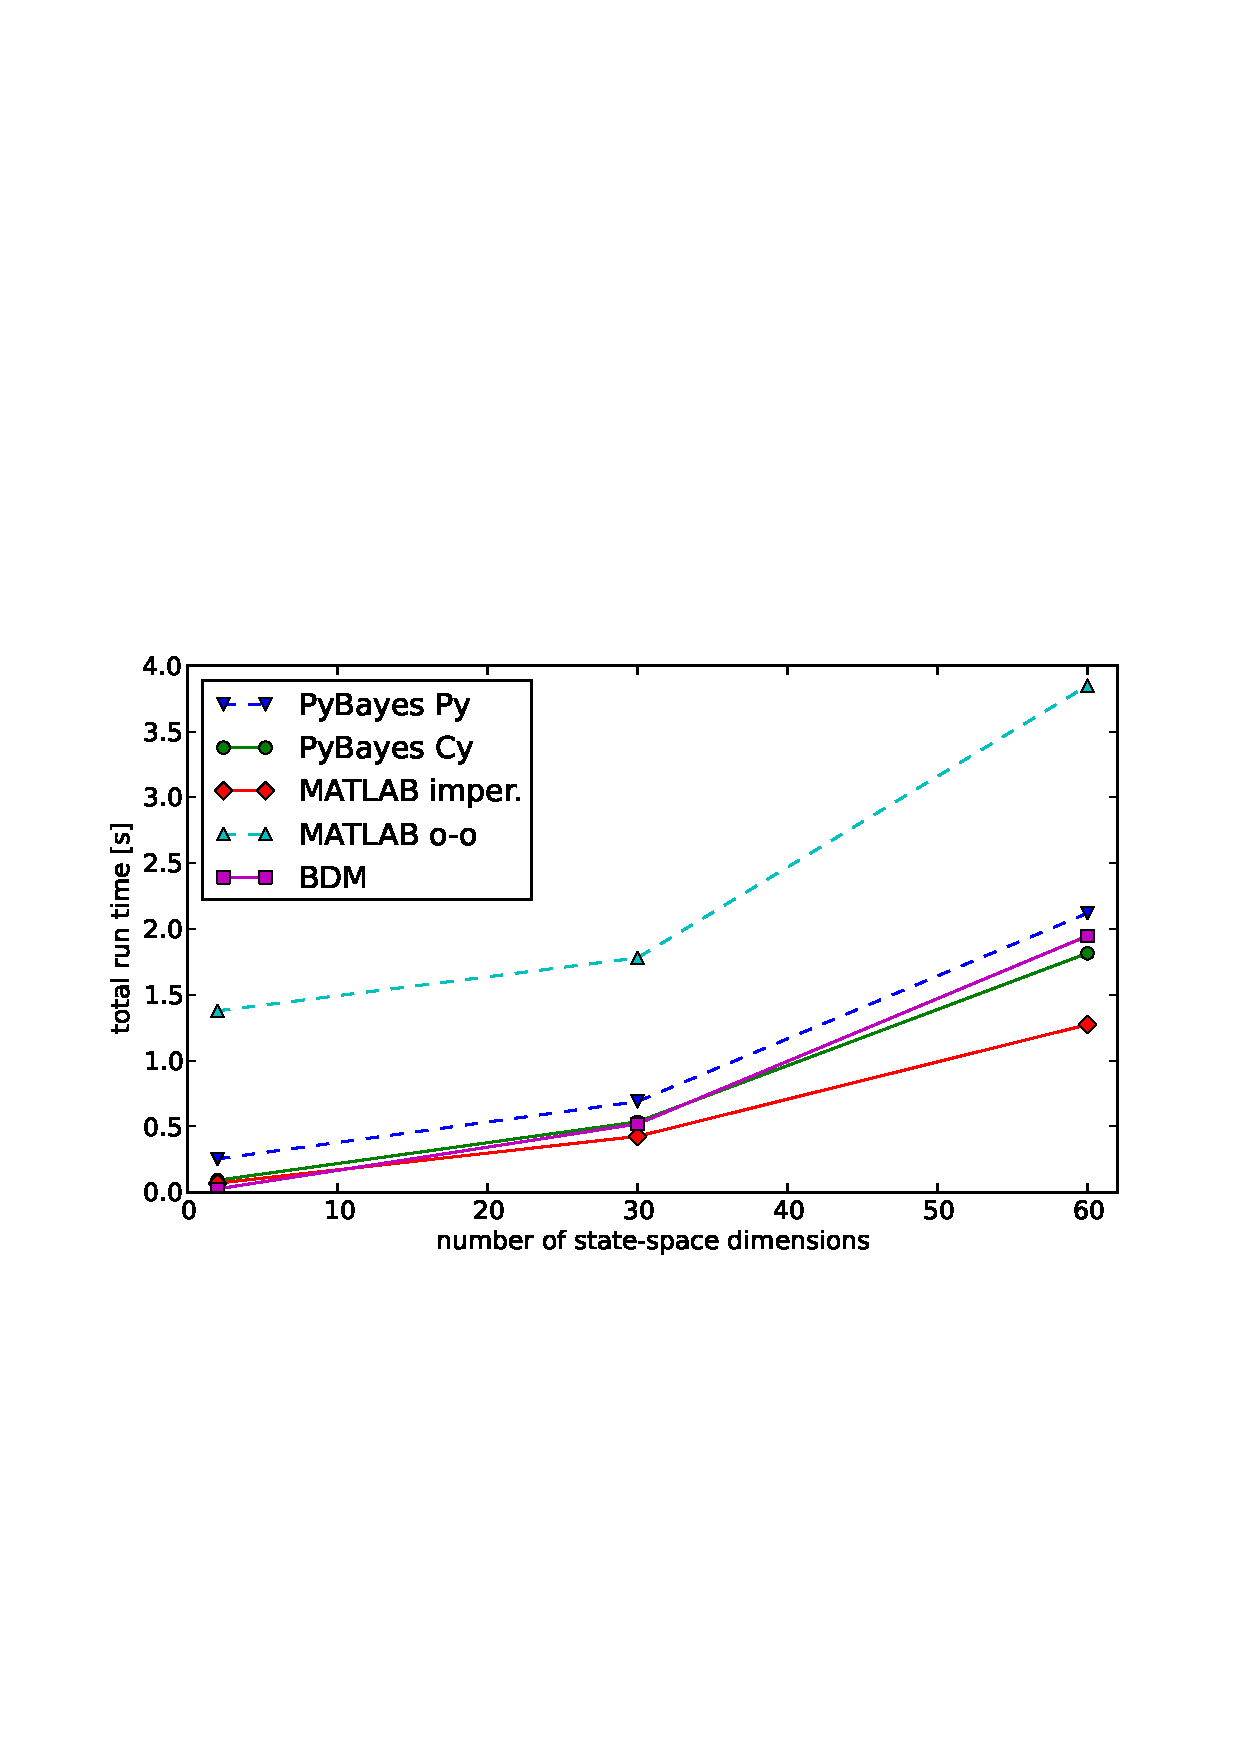
\includegraphics[width=14cm,keepaspectratio=true,clip=true,trim=19mm 85mm 20mm 111mm]{./KFPerf.pdf}
%	\vspace{-8mm}
	\caption{Run time against dimensionality of various Kalman filter implementations}
	\label{fig:KFPerf}
\end{figure}


\chapter*{Conclusion} \addcontentsline{toc}{chapter}{Conclusion}


% použitá literatura
\clearpage % so that the contents link mentions correct page
\phantomsection % so that hyperref makes correct reference
\addcontentsline{toc}{chapter}{\bibname}
\bibliographystyle{plain}
\bibliography{bibliography}

\ifrelease
	% přílohy
	\appendix % aby LaTeX cisloval jinak
	\clearpage % so that the contents link mentions correct page
	\phantomsection % so that hyperref makes correct reference
	\addcontentsline{toc}{chapter}{\appendixname}

	\part*{\appendixname}

	
\includepdf[pages=-]{../doc/_build/latex/PyBayes.pdf}
\fi

\end{document}
